\documentclass{report}
\usepackage[utf8]{inputenc}
\usepackage[italian]{babel}
\usepackage[T1]{fontenc}

\usepackage{natbib}
\usepackage{graphicx}

\usepackage{blindtext}
\usepackage{hyperref}


\title{
    
\includegraphics[width=1\textwidth]{/Users/matt/Projects/GITHUB/Documentazione/unisalento logo.png} \\
    \huge {Progetto per Principi di Ingegneria dell'Informazione} \\
}

\author{Aprile Matteo, Goffredo Filippo}
\date{2020/2021}

\begin{document}

    
    \maketitle
    \tableofcontents

    \part{Analisi dei requisiti}
    \chapter{Generale}

\section{Login}
\begin{itemize}
    \item \textbf{attore}: Amministratore, Manager, Utente acquirente
    \item \textbf{precondizione}: L’utente è già registrato
    
    \begin{enumerate}
        \item L’utente accede all’area di login
        \item L’utente inserisce username e password
        \item Il sistema verifica la correttezza delle credenziali
		\label{login1}        
		\item Il sistema torna alla Home
    \end{enumerate}

    \item \textbf{estensioni}:
	\begin {enumerate}
		\item[\ref{login1}a.] Le credenziali non sono corrette:
		
		\item Il sistema chiede il reinserimento delle credenziali
	\end{enumerate}

	\item \textbf{postcondizione}: L’utente ha effettuato il login con successo
\end{itemize}


\section{Consultare catalogo}
\begin{itemize}
    \item \textbf{attore}: Utente acquirente, Utente guest, Amministratore, Manager
	\item \textbf{precondizione}: L’utente effettua il Login

    \begin{enumerate}
        \item L’utente accede alla Home
        \item Il sistema apre il catalogo
        \item L’utente cerca, dall’apposita barra, l’articolo desiderato
        \label{catalog1}
		\item L’utente, tramite l'anteprima dell’articolo, consulta il costo
		\label{catalog2}
		\item L’utente, tramite l'anteprima dell’articolo, consulta la disponibilità
		\label{catalog3}
	\end{enumerate}

	\item \textbf{estensioni}:
	\begin{enumerate}
		\item[\ref{catalog1}a.] Il sistema non trova l’articolo
            
		\item Il sistema comunica che il nome cercato non corrisponde a nessun articolo presente nel database
	\end{enumerate}

    \item \textbf{attore}: Utente acquirente

	\item \textbf{estensioni}:
	\begin{enumerate}
		\item[\ref{catalog2}a.] La disponibilità manca
            
		\item L’utente acquirente potrà prenotare l’articolo
	\end{enumerate}

	\item \textbf{attore}: Manager
	\item \textbf{estensioni}:
        
	\begin{enumerate}
		\item[\ref{catalog3}a.] La disponibilità manca
            
		\item Il sistema comunica che manca la disponibilità tramite il numero 0
        \item Il Manager fornisce il magazzino 
	\end{enumerate}

	\item \textbf{postcondizione}: n/a
\end{itemize}
    \chapter{Amministratore}
		
\section{Creazione di un articolo}
\begin{itemize}
    \item \textbf{attore}: Amministratore
    \item \textbf{precondizione}: L’amministratore deve effettuare il Login
    
    \begin{enumerate}
        \item L’amministratore accede alla menu bar
        \label{itemCr1}
        \item L’amministratore seleziona la voce “articoli”
        \item Il sistema apre l’elenco degli articoli
        \item L’amministratore clicca sul pulsante “crea”
        \item Il sistema richiede i dati dell’articolo
    
		\begin{itemize}
        	\item PRODOTTO / COMPOSIZIONE DI PRODOTTI:
        	
			\begin{enumerate}
				\item nome
				\item immagini rappresentative
				\item descrizione max 255 char
				\item produttore
				\item costo
				\item collocazione nel magazzino self-service (corsia,scaffale)
				\item categoria
				\item sottocategoria
				\item uno o più prodotti al suo interno
			\end{enumerate}
		\end{itemize}

    
		\begin{itemize}
			\item SERVIZIO:
			
			\begin{enumerate}
				\item nome
    			\item immagini rappresentative
    			\item descrizione max 255 char
    			\item fornitore
    			\item costo
    			\item categoria
			\end{enumerate}
		\end{itemize}
    
    	\item L’amministratore inserisce i dati dell’articolo
    	\item L’amministratore clicca sul pulsante “crea”
    	\label{itemCr2}
    	\item Il sistema verifica i dati dell’articolo
    	\label{itemCr3}
    	\item Il sistema chiede la conferma della creazione
    	\item L’amministratore clicca su “conferma”
    	\item Il sistema memorizza i dati dell’articolo
    \end{enumerate}

    \item \textbf{estensioni}:
    \begin{enumerate}
		\item[\ref{itemCr1}a.] L’amministratore è appena entrato nel software
		\item Il sistema gli apre direttamente la schermata degli articoli
	\end{enumerate}
        
	\begin{enumerate}
		\item[\ref{itemCr2}a.] L’articolo inserito già esiste
		\item Il sistema chiede il reinserimento dei dati
	\end{enumerate}
        
	\begin{enumerate}
		\item[\ref{itemCr3}a.] L’amministratore non ha inserito dei dati
		\item Il sistema chiede l’inserimento dei dati mancanti
	\end{enumerate}	
            
    \item \textbf{postcondizione}: L’amministratore ha inserito un nuovo articolo nel catalogo
\end{itemize}
		

\section{Modifica di un articolo}
\begin{itemize}
	\item \textbf{attore}: Amministratore
	\item \textbf{precondizione}: L’amministratore deve effettuare il Login

	\begin{enumerate}
		\item L’amministratore accede alla menu bar
		\label{itemMod1}
		\item L’amministratore seleziona la voce “articoli”
		\item Il sistema apre l’elenco degli articoli
		\item L’amministratore clicca col tasto destro sull’articolo
		\item L’amministratore, dal menu a tendina, sceglie l’opzione “modifica”
		\item Il sistema mostra i dati dell’articolo
		\item L’amministratore modifica i dati dell’articolo
		\item L’amministratore clicca sul pulsante “modifica”
		\label{itemMod2}
		\item Il sistema verifica i dati dell’articolo
		\item Il sistema chiede la conferma della modifica
		\item L’amministratore clicca su “conferma”
		\item Il sistema memorizza i dati dell’articolo
	\end{enumerate}

	\item \textbf{estensioni}:
	\begin{enumerate}
		\item[\ref{itemMod1}a.] L’amministratore è appena entrato nel software
		\item Il sistema gli apre direttamente la schermata degli articoli
	\end{enumerate}

	\begin{enumerate}
		\item[\ref{itemMod2}a.] L’articolo inserito già esiste
		\item Il sistema chiede il reinserimento dei dati
	\end{enumerate}

	\item \textbf{postcondizione}: L’amministratore ha modificato un articolo nel catalogo
\end{itemize}


\section{Cancellazione di un articolo}
\begin{itemize}
	\item \textbf{attore}: Amministratore
	\item \textbf{precondizione}: L’amministratore deve effettuare il login
	
	\begin{enumerate}
		\item L’amministratore accede alla menu bar
		\label{itemDel1}
		\item L’amministratore seleziona la voce “articoli”
		\item Il sistema apre l’elenco degli articoli
		\item L’amministratore clicca col tasto destro sull’articolo
		\item L’amministratore, dal menu a tendina, sceglie l’opzione “cancella”
		\item Il sistema chiede la conferma della cancellazione
		\item L’amministratore clicca su “conferma”
	\end{enumerate}

	\item \textbf{estensioni}:
	\begin{enumerate}
		\item[\ref{itemDel1}a.] L’amministratore è appena entrato nel software
		\item Il sistema gli apre direttamente la schermata degli articoli
	\end{enumerate}

	\item \textbf{postcondizione}: L’amministratore ha eliminato un articolo
\end{itemize}

		
\section{Creazione di un produttore}
\begin{itemize}
	\item \textbf{attore}: Amministratore
	\item \textbf{precondizione}: L’amministratore deve effettuare il login

	\begin{enumerate}
		\item L’amministratore accede alla menu bar
		\item L’amministratore seleziona la voce “produttori”
		\item Il sistema apre l’elenco dei produttori
		\item L’amministratore clicca sul pulsante “crea”
		\item Il sistema richiede i dati del produttore
		\begin{enumerate}
			\item nome, email, telefono, sito web, città, nazione
		\end{enumerate}
		\item L’amministratore inserisce i dati del produttore
		\item L’amministratore clicca sul pulsante “crea”
		\label{prodCr1}
		\item Il sistema verifica i dati del produttore
		\item Il sistema chiede la conferma della creazione
		\item L’amministratore clicca su “conferma”
		\item Il sistema memorizza i dati del produttore
	\end{enumerate}

	\item \textbf{estensioni}:
	\begin{enumerate}
		\item[\ref{prodCr1}a.] I dati inseriti già esistono
		\item Il sistema chiede il reinserimento dei dati
	\end{enumerate}

	\item \textbf{postcondizione}: L’amministratore ha inserito un nuovo produttore
\end{itemize}

		
\section{Modifica di un produttore}
\begin{itemize}
	\item \textbf{attore}: Amministratore
	\item \textbf{precondizione}: L’amministratore deve effettuare il Login

	\begin{enumerate}
		\item L’amministratore accede alla menu bar
		\item L’amministratore seleziona la voce “produttori”
		\item Il sistema apre l’elenco dei produttori
		\item L’amministratore clicca col tasto destro sul produttore
		\item L’amministratore, dal menu a tendina, sceglie l’opzione “modifica”
		\item Il sistema mostra i dati del produttore
		\item L’amministratore modifica i dati del produttore
		\item L’amministratore clicca sul pulsante “modifica”
		\label{prodMod1}
		\item Il sistema verifica i dati del produttore
		\item Il sistema chiede la conferma della modifica
		\item L’amministratore clicca su “conferma”
		\item Il sistema memorizza i dati del produttore
	\end{enumerate}

	\item \textbf{estensioni}:
	\begin{enumerate}
		\item[\ref{prodMod1}a.] I dati inseriti già esiste
		\item Il sistema chiede il reinserimento dei dati
	\end{enumerate}

	\item \textbf{postcondizione}: L’amministratore ha modificato un produttore
\end{itemize}
		

\section{Cancellazione di un produttore}
\begin{itemize}
	\item \textbf{attore}: Amministratore
	\item \textbf{precondizione}: L’amministratore deve effettuare il login
	
	\begin{enumerate}
		\item L’amministratore accede alla menu bar
		\item L’amministratore seleziona la voce “produttori”
		\item Il sistema apre l’elenco dei produttore
		\item L’amministratore clicca col tasto destro sul produttore
		\item L’amministratore, dal menu a tendina, sceglie l’opzione “cancella”
		\item Il sistema chiede la conferma della cancellazione
		\item L’amministratore clicca su “conferma”
	\end{enumerate}

	\item \textbf{postcondizione}: L’amministratore ha eliminato un produttore
\end{itemize}


\section{Creazione di un fornitore}
\begin{itemize}
	\item \textbf{attore}: Amministratore
	\item \textbf{precondizione}: L’amministratore deve effettuare il login
	
	\begin{enumerate}
		\item L’amministratore accede alla menu bar
		\item L’amministratore seleziona la voce “fornitori”
		\item Il sistema apre l’elenco dei fornitori
		\item L’amministratore clicca sul pulsante “crea”
		\item Il sistema richiede i dati del fornitore
		\begin{enumerate}
			\item nome, email, telefono, sito web, città, nazione
		\end{enumerate}
		\item L’amministratore inserisce i dati del fornitore
		\item L’amministratore clicca sul pulsante “crea”
		\label{forCr1}
		\item Il sistema verifica i dati del fornitore
		\item Il sistema chiede la conferma della creazione
		\item L’amministratore clicca su “conferma”
		\item Il sistema memorizza i dati del fornitore
	\end{enumerate}

	\item \textbf{estensioni}:
	\begin{enumerate}
		\item[\ref{forCr1}a.] I dati inseriti già esistono 
		\item Il sistema chiede il reinserimento dei dati
	\end{enumerate}

	\item \textbf{postcondizione}: L’amministratore ha inserito un nuovo fornitore
\end{itemize}
		

\section{Modifica di un fornitore}
\begin{itemize}
	\item \textbf{attore}: Amministratore
	\item \textbf{precondizione}: L’amministratore deve effettuare il Login
	
	\begin{enumerate}
		\item L’amministratore accede alla menu bar
		\item L’amministratore seleziona la voce “fornitori”
		\item Il sistema apre l’elenco dei fornitori
		\item L’amministratore clicca col tasto destro sul fornitore
		\item L’amministratore, dal menu a tendina, sceglie l’opzione “modifica”
		\item Il sistema mostra i dati sul fornitore
		\item L’amministratore modifica i dati sul fornitore
		\item L’amministratore clicca sul pulsante “modifica”
		\label{forMod1}
		\item Il sistema verifica i dati del fornitore
		\item Il sistema chiede la conferma della modifica
		\item L’amministratore clicca su “conferma”
		\item Il sistema memorizza i dati del fornitore
	\end{enumerate}

	\item \textbf{estensioni}:
	\begin{enumerate}
		\item[\ref{forMod1}a.] I dati inseriti già esistono
		\item Il sistema chiede il reinserimento dei dati
	\end{enumerate}

	\item \textbf{postcondizione}: L’amministratore ha modificato un fornitore
\end{itemize}
		

\section{Cancellazione di un fornitore}
\begin{itemize}
	\item \textbf{attore}: Amministratore
	\item \textbf{precondizione}: L’amministratore deve effettuare il login

	\begin{enumerate}
		\item L’amministratore accede alla menu bar
		\item L’amministratore seleziona la voce “fornitori”
		\item Il sistema apre l’elenco dei fornitori
		\item L’amministratore clicca col tasto destro sul fornitore
		\item L’amministratore, dal menu a tendina, sceglie l’opzione “cancella”
		\item Il sistema chiede la conferma della cancellazione
		\item L’amministratore clicca su “conferma”
	\end{enumerate}

	\item \textbf{postcondizione}: L’amministratore ha eliminato un fornitore
\end{itemize}


\section{Creazione di una categoria}
\begin{itemize}
	\item \textbf{attore}: Amministratore
	\item \textbf{precondizione}: L’amministratore deve effettuare il login
	
	\begin{enumerate}
		\item L’amministratore accede alla menu bar
		\item L’amministratore seleziona la voce “categorie”
		\item Il sistema apre l’elenco delle categorie
		\item L’amministratore clicca sul pulsante “crea”
		\item Il sistema richiede i dati della categoria
		\item L’amministratore inserisce i dati della categoria
		\item L’amministratore clicca sul pulsante “crea”
		\label{catCr1}
		\item Il sistema verifica i dati della categoria
		\item Il sistema chiede la conferma della creazione
		\item L’amministratore clicca su “conferma”
		\item Il sistema memorizza i dati della categoria
	\end{enumerate}

	\item \textbf{estensioni}:
	\begin{enumerate}
		\item[\ref{catCr1}a.] I dati inseriti già esistono 
		\item Il sistema chiede il reinserimento dei dati
	\end{enumerate}

	\item \textbf{postcondizione}: L’amministratore ha inserito una nuova categoria
\end{itemize}


\section{Modifica di una categoria}
\begin{itemize}
	\item \textbf{attore}: Amministratore
	\item \textbf{precondizione}: L’amministratore deve effettuare il Login
	
	\begin{enumerate}
		\item L’amministratore accede alla menu bar
		\item L’amministratore seleziona la voce “categorie”
		\item Il sistema apre l’elenco delle categorie
		\item L’amministratore clicca col tasto destro sulla categoria
		\item L’amministratore, dal menu a tendina, sceglie l’opzione “modifica”
		\item Il sistema mostra i dati sulla categoria
		\item L’amministratore modifica i dati sulla categoria
		\item L’amministratore clicca sul pulsante “modifica”
		\label{catMod1}
		\item Il sistema verifica i dati della categoria
		\item Il sistema chiede la conferma della modifica
		\item L’amministratore clicca su “conferma”
		\item Il sistema memorizza i dati della categoria
	\end{enumerate}

	\item \textbf{estensioni}:
	\begin{enumerate}
		\item[\ref{catMod1}a.] I dati inseriti già esistono
		\item Il sistema chiede il reinserimento dei dati
	\end{enumerate}

	\item \textbf{postcondizione}: L’amministratore ha modificato una categoria
\end{itemize}


\section{Cancellazione di una categoria}
\begin{itemize}
	\item \textbf{attore}: Amministratore
	\item \textbf{precondizione}: L’amministratore deve effettuare il login
	
	\begin{enumerate}
		\item L’amministratore accede alla menu bar
		\item L’amministratore seleziona la voce “categorie”
		\item Il sistema apre l’elenco delle categorie
		\item L’amministratore clicca col tasto destro sulla categoria
		\item L’amministratore, dal menu a tendina, sceglie l’opzione “cancella”
		\item Il sistema chiede la conferma della cancellazione
		\item L’amministratore clicca su “conferma”
	\end{enumerate}

	\item \textbf{postcondizione}: L’amministratore ha eliminato una categoria
\end{itemize}


\section{Creazione di una sottocategoria}
\begin{itemize}
	\item \textbf{attore}: Amministratore
	\item \textbf{precondizione}: L’amministratore deve effettuare il login

	\begin{enumerate}
		\item L’amministratore accede alla menu bar
		\item L’amministratore seleziona la voce “categorie”
		\item Il sistema apre l’elenco delle categorie
		\item L’amministratore clicca col tasto destro sull’articolo
		\item L’amministratore, dal menu a tendina, sceglie l’opzione “modifica”
		\item Il sistema mostra i dati della categoria
		\item L’amministratore clicca sul pulsante “+”
		\label{scatCr1}
		\item Il sistema richiede il nome della sottocategoria
		\item L’amministratore inserisce i dati della sottocategoria
		\item L’amministratore clicca sul pulsante “crea”
		\item Il sistema verifica i dati della sottocategoria
		\item Il sistema chiede la conferma della creazione
		\item L’amministratore clicca su “conferma”
		\item Il sistema memorizza i dati della sottocategoria
	\end{enumerate}

	\item \textbf{estensioni}:
	\begin{enumerate}
		\item[\ref{scatCr1}a.] La sottocategoria già esiste
		\item Il sistema chiede il reinserimento del nome
	\end{enumerate}

	\item \textbf{postcondizione}: L’amministratore ha inserito una nuova sottocategoria	
\end{itemize}


\section{Creazione punto vendita}
\begin{itemize}
	\item \textbf{attore}: Amministratore
	\item \textbf{precondizione}: L’amministratore deve effettuare il login
	
	\begin{enumerate}
		\item L’amministratore accede alla menu bar
		\item L’amministratore seleziona la voce “punti vendita”
		\item Il sistema apre l’elenco dei punti vendita
		\item L’amministratore clicca sul pulsante “crea”
		\item Il sistema richiede i dati del punto vendita
		\begin{enumerate}
			\item nome, categorie di articoli venduti, manager, posizione ...
		\end{enumerate}
		\item L’amministratore inserisce i dati del punto vendita
		\item L’amministratore clicca sul pulsante “crea”
		\item Il sistema verifica i dati del punto vendita
		\label{storeCr1}
		\item Il sistema chiede la conferma del punto vendita
		\item L’amministratore clicca su “conferma”
		\item Il sistema memorizza i dati del punto vendita
	\end{enumerate}

	\item \textbf{estensioni}:
	\begin{enumerate}
		\item[\ref{storeCr1}a.] I dati inseriti già esistono 
		\item Il sistema chiede il reinserimento dei dati
	\end{enumerate}

	\item \textbf{postcondizione}: L’amministratore ha inserito un nuovo punto vendita
\end{itemize}


\section{Modifica di un punto vendita}
\begin{itemize}
	\item \textbf{attore}: Amministratore
	\item \textbf{precondizione}: L’amministratore deve effettuare il Login
	
	\begin{enumerate}
		\item L’amministratore accede alla menu bar
		\item L’amministratore seleziona la voce “punti vendita”
		\item Il sistema apre l’elenco dei punti vendita
		\item L’amministratore clicca col tasto destro sul punto  vendita
		\item L’amministratore, dal menu a tendina, sceglie l’opzione “modifica”
		\item Il sistema mostra i dati del punto vendita
		\item L’amministratore modifica i dati sul punto vendita
		\item L’amministratore clicca sul pulsante “modifica”
		\label{storeMod1}
		\item Il sistema verifica i dati del punto vendita
		\item Il sistema chiede la conferma del punto vendita
		\item L’amministratore clicca su “conferma”
		\item Il sistema memorizza i dati del punto vendita
	\end{enumerate}

	\item \textbf{estensioni}:
	\begin{enumerate}
		\item[\ref{storeMod1}a.] I dati inseriti già esistono
		\item Il sistema chiede il reinserimento dei dati
	\end{enumerate}

	\item \textbf{postcondizione}: L’amministratore ha modificato un punto vendita
\end{itemize}


\section{Cancellazione di un punto vendita}
\begin{itemize}
	\item \textbf{attore}: Amministratore
	\item \textbf{precondizione}: L’amministratore deve effettuare il login
	
	\begin{enumerate}
		\item L’amministratore accede alla menu bar
		\item L’amministratore seleziona la voce “punti vendita”
		\item Il sistema apre l’elenco dei punti vendita
		\item L’amministratore clicca col tasto destro sul punto vendita
		\item L’amministratore, dal menu a tendina, sceglie l’opzione “cancella”
		\item Il sistema chiede la conferma della cancellazione
		\item L’amministratore clicca su “conferma”
	\end{enumerate}

	\item \textbf{postcondizione}: L’amministratore ha eliminato un punto vendita
\end{itemize}


\section{Creazione di un Manager}
\begin{itemize}
	\item \textbf{attore}: Amministratore
	\item \textbf{precondizione}:  L’amministratore deve effettuare il login
	
	\begin{enumerate}
		\item L’amministratore accede alla menu bar
		\item L’amministratore seleziona la voce “manager”
		\item Il sistema apre l’elenco dei Manager
		\item L’amministratore clicca sul pulsante “crea”
		\item Il sistema richiede i dati del Manager
		\item L’amministratore inserisce i dati del Manager
		\item L’amministratore clicca sul pulsante “crea”
		\label{manCr1}
		\item Il sistema verifica i dati del Manager
		\item Il sistema chiede la conferma del Manager
		\item L’amministratore clicca su “conferma”
		\item Il sistema memorizza i dati del Manager
	\end{enumerate}

	\item \textbf{estensioni}:
	\begin{enumerate}
		\item[\ref{manCr1}a.] I dati inseriti già esistono 
		\item Il sistema chiede il reinserimento dei dati
	\end{enumerate}

	\item \textbf{postcondizione}: L’amministratore ha inserito un nuovo Manager
\end{itemize}

		
\section{Modifica di un Manager}
\begin{itemize}
	\item \textbf{attore}: Amministratore
	\item \textbf{precondizione}: L’amministratore deve effettuare il Login
	
	\begin{enumerate}
		\item L’amministratore accede alla menu bar
		\item L’amministratore seleziona la voce “Manager”
		\item Il sistema apre l’elenco dei Manager
		\item L’amministratore clicca col tasto destro sul Manager
		\item L’amministratore, dal menu a tendina, sceglie l’opzione “modifica”
		\item Il sistema mostra i dati del Manager
		\item L’amministratore modifica i dati sul Manager
		\item L’amministratore clicca sul pulsante “modifica”
		\label{manMod1}
		\item Il sistema verifica i dati del Manager
		\item Il sistema chiede la conferma del Manager
		\item L’amministratore clicca su “conferma”
		\item Il sistema memorizza i dati del Manager
	\end{enumerate}

	\item \textbf{estensioni}:
	\begin{enumerate}
		\item[\ref{manMod1}a.] I dati inseriti già esistono
		\item Il sistema chiede il reinserimento dei dati
	\end{enumerate}

	\item \textbf{postcondizione}: L’amministratore ha modificato un Manager
\end{itemize}

		
\section{Cancellazione di un Manager}
\begin{itemize}
	\item \textbf{attore}: Amministratore
	\item \textbf{precondizione}: L’amministratore deve effettuare il login
	
	\begin{enumerate}
		\item L’amministratore accede alla menu bar
		\item L’amministratore seleziona la voce “Manager”
		\item Il sistema apre l’elenco dei Manager
		\item L’amministratore clicca col tasto destro sul Manager
		\item L’amministratore, dal menu a tendina, sceglie l’opzione “cancella”
		\item Il sistema chiede la conferma della cancellazione
		\item L’amministratore clicca su “conferma”
	\end{enumerate}

	\item \textbf{postcondizione}: L’amministratore ha eliminato un Manager
\end{itemize}
    \chapter{Manager}

\section{Creazione di un ordine}
\begin{itemize}
    \item \textbf{attore}: Manager
    \item \textbf{precondizione}: Il Manager deve effettuare il login

    \begin{enumerate}
        \item Il Manager accede alla menu bar
        \item Il Manager seleziona la voce “articoli”
        \item Il sistema apre l’elenco degli articoli
        \item Il Manager cerca, dall’apposita barra, l’articolo desiderato
        \item Il sistema trova l’articolo
        \label{orderCr1}
        \item Il Manager inserisce la quantità nell’apposito spazio
        \item Il Manager clicca sul pulsante “+”
        \item Il sistema aggiunge l’articolo all’ordine
    \end{enumerate}

    \item \textbf{estensioni}:
    \begin{enumerate}
        \item[\ref{orderCr1}a.] Il sistema non trova gli articoli
        \item Il sistema comunica che il nome cercato non corrisponde a nessun articolo presente nel database
    \end{enumerate}

    \item \textbf{postcondizione} Il Manager ha creato un ordine
\end{itemize}


\section{Modifica di un ordine}
\begin{itemize}
    \item \textbf{attore}: Manager
    \item \textbf{precondizione}: Il Manager deve effettuare il Login

    \begin{enumerate}
        \item L’amministratore accede alla menu bar
        \item L’amministratore seleziona la voce “Manager”
        \item Il sistema apre l’elenco dei Manager
        \item L’amministratore clicca col tasto destro sul Manager
        \item L’amministratore, dal menu a tendina, sceglie l’opzione “modifica”
        \item Il sistema mostra i dati del Manager
        \item L’amministratore modifica i dati sul Manager
        \item L’amministratore clicca sul pulsante “modifica”
        \label{orderMod1}
        \item Il sistema verifica i dati del Manager
        \item Il sistema chiede la conferma del Manager
        \item L’amministratore clicca su “conferma”
        \item Il sistema memorizza i dati del Manager
    \end{enumerate}

    \item \textbf{estensioni}:
    \begin{enumerate}
        \item[\ref{orderMod1}a.] I dati inseriti già esistono
        \item Il sistema chiede il reinserimento dei dati
    \end{enumerate}

    \item \textbf{postcondizione}: Il Manager ha modificato un ordine
\end{itemize}


\section{Cancellazione di un ordine}
\begin{itemize}
    \item \textbf{attore}: Manager
    \item \textbf{precondizione}: Il Manager deve effettuare il login

    \begin{enumerate}
        \item Il Manager accede alla menu bar
        \item Il Manager seleziona la voce “ordine”
        \item Il sistema apre l’elenco degli ordini
        \item Il Manager clicca sul tasto “-”
        \item Il sistema chiede la conferma della cancellazione
        \item Il Manager clicca su “conferma”
    \end{enumerate}

    \item \textbf{postcondizione}: Il Manager ha eliminato un ordine
\end{itemize}


\section{Effettuare pagamento}
\begin{itemize}
    \item \textbf{attore}: Manager
    \item \textbf{precondizione}: Creazione di un ordine
    
    \begin{enumerate}
        \item Il Manager accede alla menu bar
        \item Il Manager clicca su “ordine”
        \item Il sistema apre l’elenco dell’ordine 
        \item Il Manager clicca su “ordina”
        \item Il sistema chiede i dati per effettuare il pagamento
        \item Il Manager inserisce i dati per il pagamento
        \item Il Manager clicca su “conferma”
        \item Il sistema verifica che i dati siano corretti
        \label{pay1}
        \item Il sistema chiede se si vuole confermare l’ordine
        \item Il Manager clicca su “conferma”
    \end{enumerate}
    
    \item \textbf{estensioni}:
    \begin{enumerate}
        \item[\ref{pay1}a.] I dati non sono corretti
        \item Il sistema richiede il reinserimento dei dati
    \end{enumerate}

    \item \textbf{postcondizione}: Il Manager ha effettuato il pagamento dell’ordine
\end{itemize}


\section{Disabilitazione di un utente}
\begin{itemize}
    \item \textbf{attore}: Manager
    \item \textbf{precondizione}: Il Manager deve effettuare il login
    
    \begin{enumerate}
        \item Il Manager accede alla menu bar
        \item Il Manager seleziona la voce “utenza”
        \item Il sistema apre l’elenco degli utenti registrati al punto vendita del Manager
        \item Il Manager cerca, dall’apposita barra, l’utente desiderato
        \item Il Manager clicca col tasto destro sull’utente
        \item Il Manager, dal menu a tendina, sceglie l’opzione “disabilita”
        \item Il sistema chiede la conferma della disabilitazione
        \item Il Manager clicca su “conferma”
    \end{enumerate}

    \item \textbf{postcondizione}: Il Manager disabilita il profilo di un utente
\end{itemize}


\section{Cancellazione di un utente}
\begin{itemize}
    \item \textbf{attore}: Manager
    \item \textbf{precondizione}: Il Manager deve effettuare il login
    
    \begin{enumerate}
        \item Il Manager accede alla menu bar
        \item Il Manager seleziona la voce “utenza”
        \item Il sistema apre l’elenco degli utenti registrati al punto vendita del Manager
        \item Il Manager cerca, dall’apposita barra, l’utente desiderato
        \item Il Manager clicca col tasto destro sull’utente
        \item Il Manager, dal menu a tendina, sceglie l’opzione “disabilita”
        \item Il sistema chiede la conferma della cancellazione
        \item Il Manager clicca su “conferma”
    \end{enumerate}

    \item \textbf{postcondizione}: Il Manager cancella il profilo di un utente
\end{itemize}


\section{Inviare un’e-mail ad un utente}
\begin{itemize}
    \item \textbf{attore}: Manager
    \item \textbf{precondizione}: Il Manager deve effettuare il login
    
    \begin{enumerate}
        \item Il Manager accede alla menu bar
        \item Il Manager seleziona la voce “utenza”
        \item Il sistema apre l’elenco degli utenti registrati al punto vendita del Manager
        \item Il Manager cerca, dall’apposita barra, l’utente desiderato
        \item Il Manager clicca col tasto destro sull’utente
        \item Il Manager, dal menu a tendina, sceglie l’opzione “invia e-mail”
        \item Il sistema richiede di inserire oggetto e messaggio
        \item Il Manager inserisce oggetto e messaggio
        \item Il Manager clicca su “invia”
        \item Il sistema invia l’email
    \end{enumerate}

    \item \textbf{postcondizione}: Il Manager ha inviato un’e-mail ad un utente
\end{itemize}


\section{Gestione dei feedback}
\begin{itemize}
    \item \textbf{attore}: Manager
    \item \textbf{precondizione}: Il Manager deve effettuare il login 
    
    \begin{enumerate}
        \item Il Manager accede alla Home
        \item Il Manager cerca, dall’apposita barra, l’articolo desiderato
        \item Il Manager clicca col tasto sinistro l’articolo interessato
        \item Il Manager scorre fino ad arrivare al feedback interessato
        \item Il Manager commenta nell’apposito spazio
    \end{enumerate}

    \item \textbf{postcondizione}: Il Manager ha potuto rispondere ad un cliente
\end{itemize}

    \chapter{Utente acquirente}


\section{Prenotazione di un articolo}
\begin{itemize}
    \item \textbf{attore}: Utente acquirente
    \item \textbf{precondizione}: L’utente acquirente effettua il login

    \begin{enumerate}
        \item L’utente acquirente accede alla Home
        \item L’utente acquirente cerca, dall’apposita barra, l’articolo desiderato
        \item L’utente acquirente clicca sull’articolo interessato
        \item L’utente acquirente clicca sul pulsante “prenota subito”
        \item Il sistema chiede la conferma della prenotazione
        \label{itemPren1}
        \item L'utente acquirente clicca su “conferma”
        \item Il sistema prenota l’articolo
    \end{enumerate}

    \item \textbf{estensioni}:
    \begin{enumerate}
        \item[\ref{itemPren1}a.] La prenotazione non può avvenire
        \item Il sistema avvisa l’utente acquirente che non è possibile prenotare l’articolo desiderato
    \end{enumerate}

    \item \textbf{postcondizione}: L’utente acquirente ha prenotato l’articolo desiderato
\end{itemize}


\section{Creazione di una lista d’acquisto}
\begin{itemize}
    \item \textbf{attore}: Utente acquirente
    \item \textbf{precondizione}: L’utente acquirente deve effettua il login

    \begin{enumerate}
        \item L’utente acquirente accede alla Home
        \item L’utente acquirente clicca sul pulsante “liste”
        \item Il sistema apre l’elenco delle liste
        \item L’utente acquirente clicca sul pulsante “crea”
        \item Il sistema richiede il nome della lista 
        \item L’utente acquirente inserisce i dati della lista
        \item L’utente acquirente clicca sul pulsante “conferma”
        \item Il sistema verifica i dati della lista
        \label{listCr1}
        \item Il sistema memorizza i dati della lista
    \end{enumerate}

    \item \textbf{estensioni}:
    \begin{enumerate}
        \item[\ref{listCr1}a.] La lista già esiste
        \item Il sistema notifica che la lista già esiste
    \end{enumerate}

    \item \textbf{postcondizione}: L’utente acquirente ha creato una nuova lista
\end{itemize}
		

\section{Modifica di una lista d’acquisto}
\begin{itemize}
    \item \textbf{attore}: Utente acquirente
    \item \textbf{precondizione}: L’utente acquirente deve effettua il login
    
    \begin{enumerate}
        \item L’utente acquirente accede alla Home
        \item L’utente acquirente clicca sul pulsante “liste”
        \item Il sistema apre l’elenco delle liste
        \item L’utente acquirente clicca sulla lista interessata
        \item Il sistema apre la lista 
        \item L’utente acquirente elimina un articolo tramite il pulsante “-”
        \item Il sistema chiede la conferma dell’eliminazione
        \item L’utente acquirente clicca sul pulsante “conferma”
        \item Il sistema cancella l’articolo dalla lista
    \end{enumerate}
    
    \item \textbf{postcondizione}: L’utente acquirente ha eliminato un articolo dalla lista
\end{itemize}


\section{Cancellazione di una lista d’acquisto}
\begin{itemize}
    \item \textbf{attore}: Utente acquirente
    \item \textbf{precondizione}: L’utente acquirente deve effettua il login
    
    \begin{enumerate}
        \item L’utente acquirente accede alla Home
        \item L’utente acquirente clicca sul pulsante “liste”
        \item Il sistema apre l’elenco delle liste
        \item L’utente acquirente elimina una lista tramite il pulsante “-”
        \item Il sistema chiede la conferma dell’eliminazione
        \item L’utente acquirente clicca sul pulsante “conferma”
        \item Il sistema cancella l’articolo dalla lista
    \end{enumerate}

    \item \textbf{postcondizione}: L’utente acquirente ha eliminato una lista
\end{itemize}
		

\section{Aggiungere un articolo in una lista d’acquisto}
\begin{itemize}
    \item \textbf{attore}: Utente acquirente
    \item \textbf{precondizione}: L’utente acquirente deve effettua il login

    \begin{enumerate}
        \item L’utente acquirente accede alla Home
        \item L’utente acquirente clicca sul pulsante “+” presente dell’anteprima dell’articolo
        \item Il sistema apre l’elenco delle liste già create
        \item L’utente acquirente sceglie la lista alla quale aggiungere l’articolo
        \label{listAdd1}
        \item Il sistema memorizza l’articolo nella lista
    \end{enumerate}

    \item \textbf{estensioni}:
    \begin{enumerate}
        \item[\ref{listAdd1}a.] La lista non esiste
        \item L’utente acquirente crea una nuova lista
    \end{enumerate}

    \item \textbf{postcondizione}:  L’utente acquirente ha creata la sua lista d’acquisto
\end{itemize}


\section{Creazione di un pdf della lista d’acquisto}
\begin{itemize}
    \item \textbf{attore}: Utente acquirente
    \item \textbf{precondizione}: L’utente acquirente deve effettuare il login
    
    \begin{enumerate}
        \item L’utente acquirente accede alla Home
        \item L’utente acquirente clicca sul pulsante “liste”
        \item Il sistema apre l’elenco delle liste
        \item L’utente acquirente clicca col tasto destro sulla lista interessata
        \item L’utente acquirente, dal menu a tendina, sceglie l’opzione “invia pdf”
        \item Il sistema crea un pdf della lista d’acquisto
        \item Il sistema spedisce via e-mail il pdf
        \item L’utente acquirente riceve l’email
    \end{enumerate}

    \item \textbf{postcondizione}: L’utente acquirente ha ricevuto il pdf della sua lista d’acquisto
\end{itemize}


\section{Rilascio di feedback}
\begin{itemize}
    \item \textbf{attore}: Utente acquirente
    \item \textbf{precondizione}: L’utente acquirente deve effettuare il login 

    \begin{enumerate}
        \item L’utente acquirente accede alla Home
        \item L’utente acquirente cerca, dall’apposita barra, l’articolo desiderato
        \item L’utente acquirente clicca col tasto sinistro l’articolo interessato
        \item L’utente acquirente scorre fino ad arrivare alla sezione feedback
        \item L’utente acquirente commenta nell’apposito spazio
    \end{enumerate}

    \item \textbf{postcondizione}: L’utente acquirente ha rilasciato un feedback
\end{itemize}

    \chapter{Utente guest}


\section{Registrazione}
\begin{itemize}
    \item \textbf{attore}: Utente Guest
    \item \textbf{precondizioni}: n/a
    
    \begin{enumerate}
        \item L’utente accede all’area di registrazione
        \item L’utente inserisce i suoi dati
        \label{reg1}
        \begin{enumerate}
            \item nome, cognome, e-mail, telefono, età, residenza, professione
        \end{enumerate}
        \item Il sistema verifica i dati non siano già esistenti
        \item Il sistema gli memorizza
        \item Il sistema torna alla Home
    \end{enumerate}

    \item \textbf{estensioni}:
    \begin{enumerate}
        \item[\ref{reg1}a.] I dati sono già esistenti
        \item Il sistema avvisa l’utente che i dati sono già esistenti
    \end{enumerate}

    \item \textbf{postcondizione}: L’utente guest si è registrato
\end{itemize}


    \part{UML dell'architettura software}
    \chapter{UML dei casi d'uso}

\includegraphics[width=\textwidth]{/Users/matt/Projects/GITHUB/Documentazione/UML dell'architettura software/UML dei casi d'uso/UML dei casi d’uso.jpg}

    \chapter{Schede CRC}

\paragraph{
    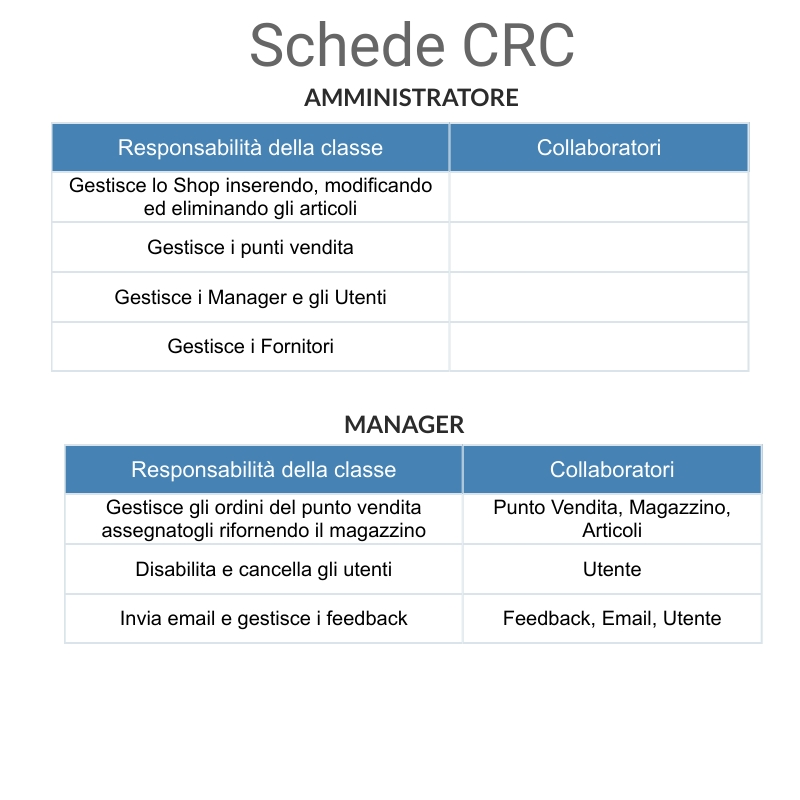
\includegraphics[width=\textwidth]{/Users/matt/Projects/GITHUB/Documentazione/UML dell'architettura software/Schede CRC/CRC1.jpg}
}

\paragraph{
    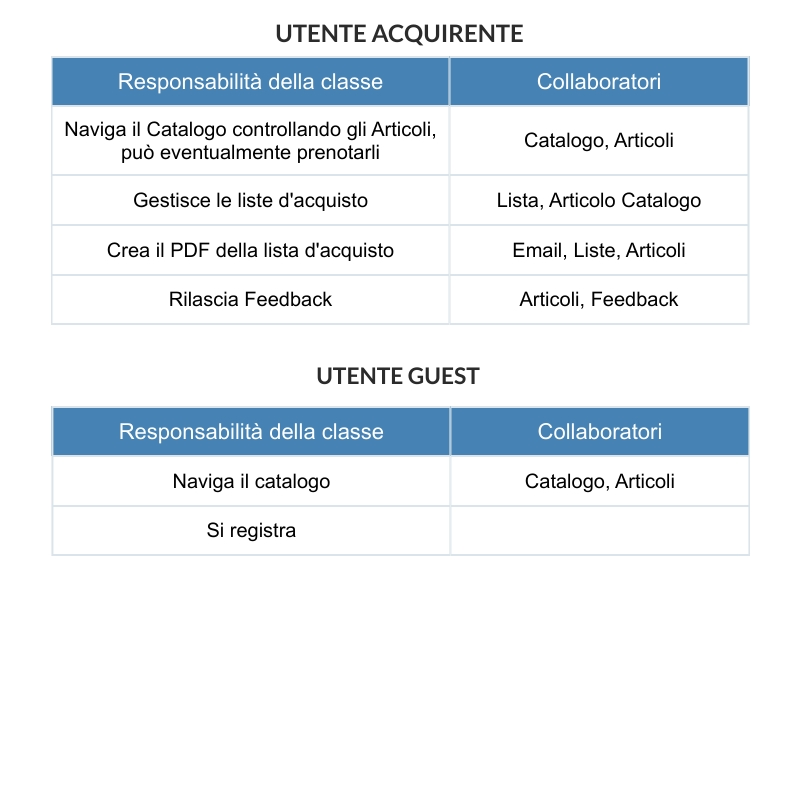
\includegraphics[width=\textwidth]{/Users/matt/Projects/GITHUB/Documentazione/UML dell'architettura software/Schede CRC/CRC2.jpg}
}

\paragraph{
    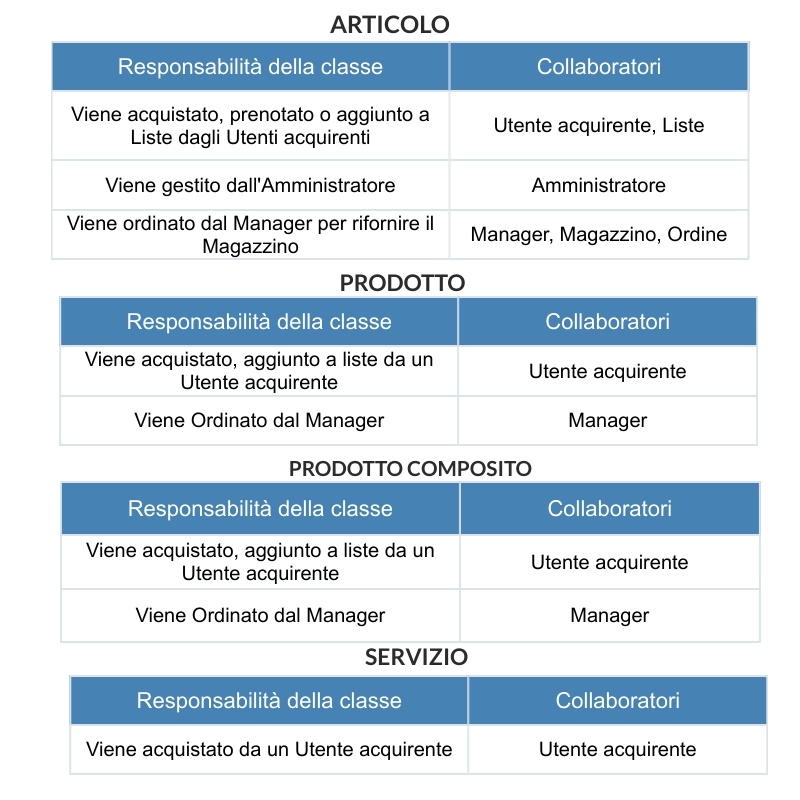
\includegraphics[width=\textwidth]{/Users/matt/Projects/GITHUB/Documentazione/UML dell'architettura software/Schede CRC/CRC3.jpg}
}

\paragraph{
    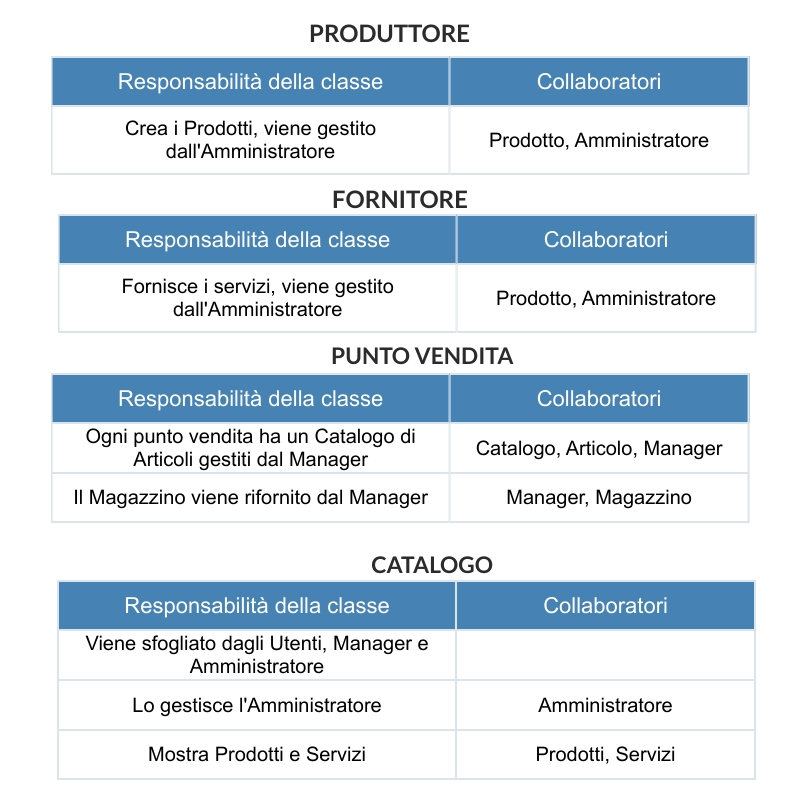
\includegraphics[width=\textwidth]{/Users/matt/Projects/GITHUB/Documentazione/UML dell'architettura software/Schede CRC/CRC4.jpg}
}

\paragraph{
    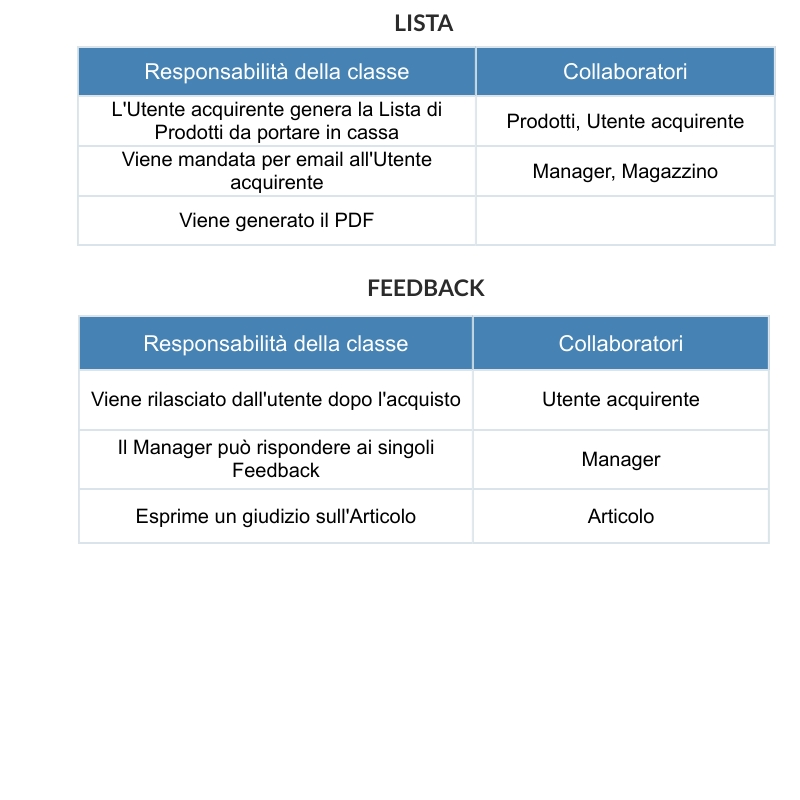
\includegraphics[width=\textwidth]{/Users/matt/Projects/GITHUB/Documentazione/UML dell'architettura software/Schede CRC/CRC5.jpg}
}
    \chapter{Diagramma delle classi}

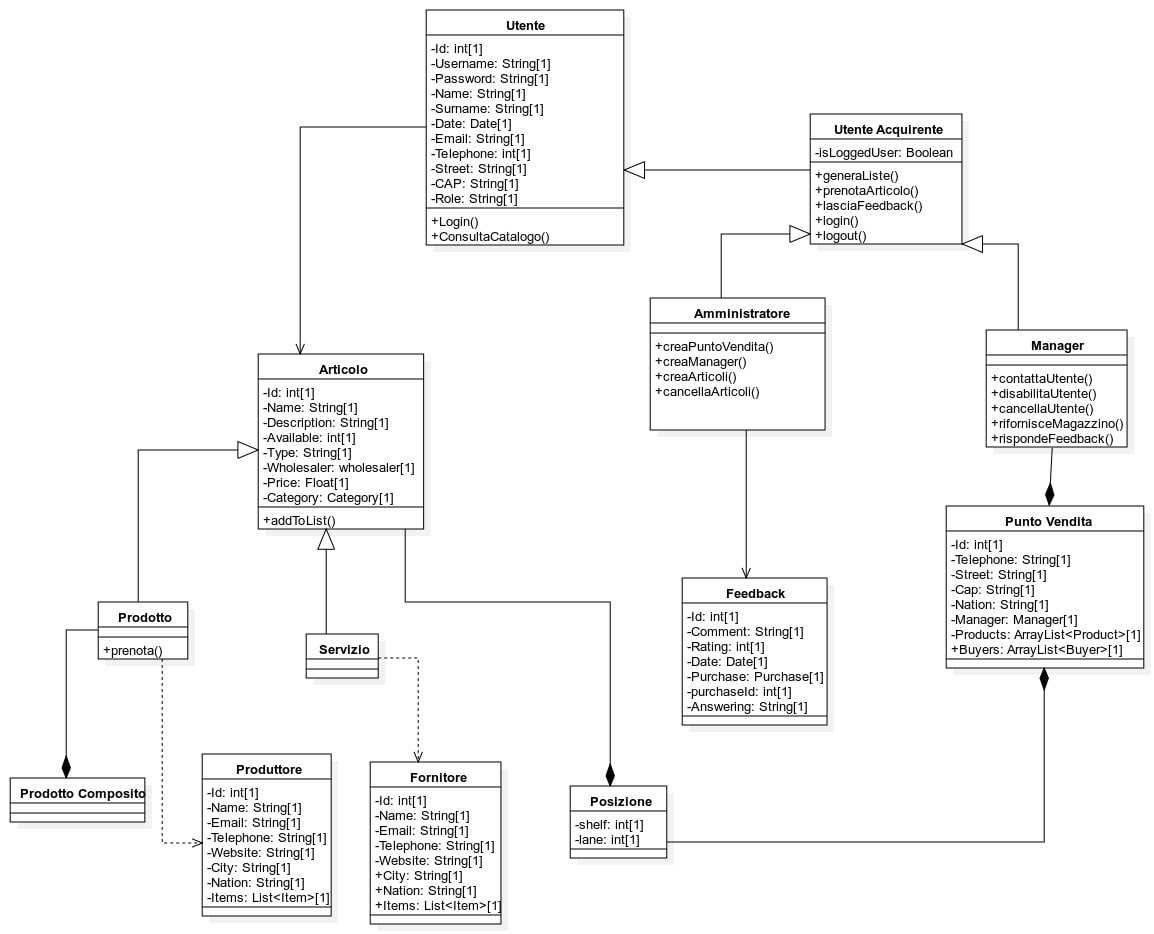
\includegraphics[width=\textwidth]{/Users/matt/Projects/GITHUB/Documentazione/UML dell'architettura software/Diagramma delle classi/ClassDiagram.jpg}

    \chapter{Diagrammi di sequenza}

\centering
\paragraph{
    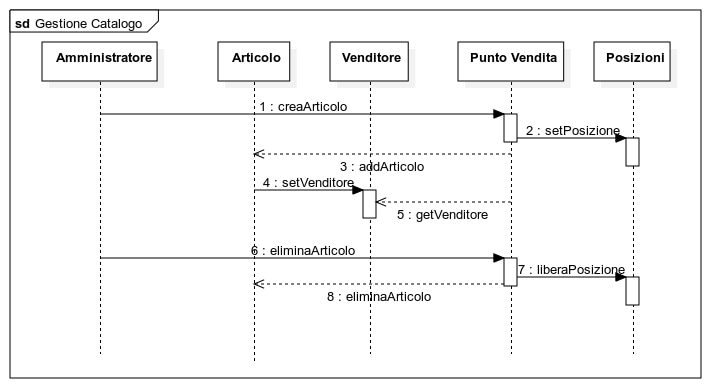
\includegraphics[width=\textwidth]{/Users/matt/Projects/GITHUB/Documentazione/UML dell'architettura software/Diagrammi di sequenza/seq1.jpg}
}

\paragraph{
    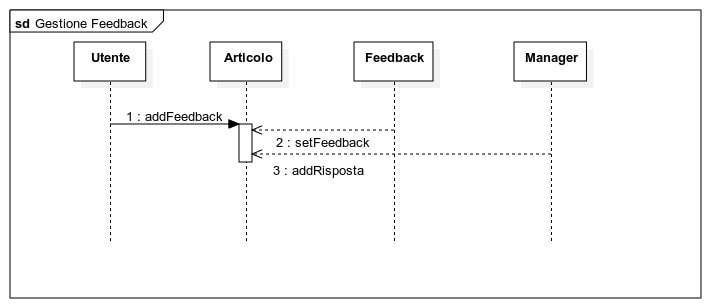
\includegraphics[width=\textwidth]{/Users/matt/Projects/GITHUB/Documentazione/UML dell'architettura software/Diagrammi di sequenza/seq2.jpg}
}

\paragraph{
    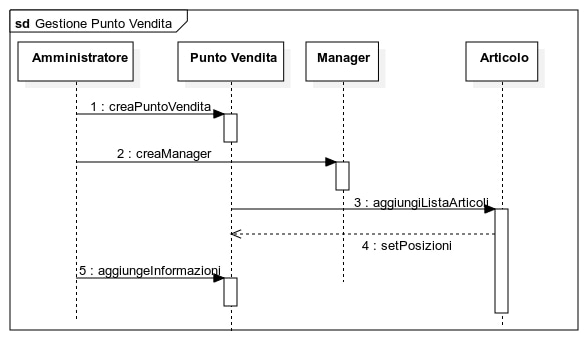
\includegraphics[width=\textwidth]{/Users/matt/Projects/GITHUB/Documentazione/UML dell'architettura software/Diagrammi di sequenza/seq3.jpg}
}

\paragraph{
    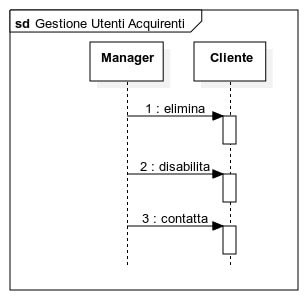
\includegraphics[width=0.6\textwidth]{/Users/matt/Projects/GITHUB/Documentazione/UML dell'architettura software/Diagrammi di sequenza/seq4.jpg}
}

\paragraph{
    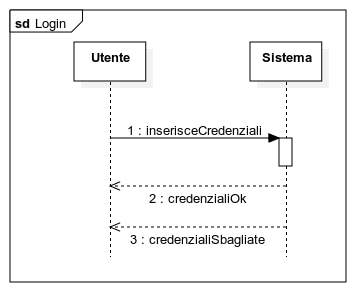
\includegraphics[width=0.6\textwidth]{/Users/matt/Projects/GITHUB/Documentazione/UML dell'architettura software/Diagrammi di sequenza/seq5.jpg}
}

\paragraph{
    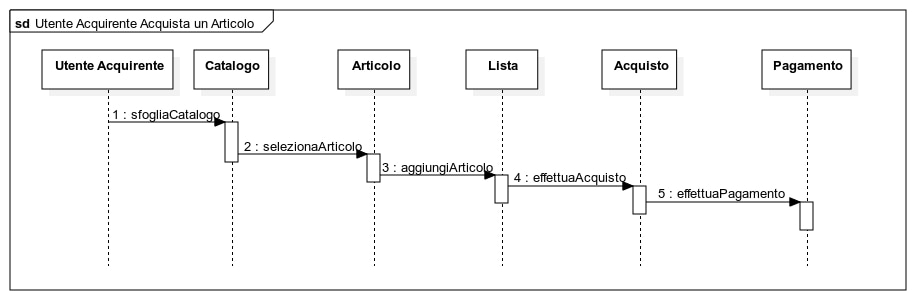
\includegraphics[width=\textwidth]{/Users/matt/Projects/GITHUB/Documentazione/UML dell'architettura software/Diagrammi di sequenza/seq6.jpg}
}

    \part{Utilizzo dei design pattern adottati}
    \chapter{Indicazione dei design pattern}

I design pattern che sono stati utilizzati all'interno per codice sono i sueguenti:

\begin{itemize}
    \item Bridge: utilizzato per isolare la libreria che ci permette di creare il pdf da mandare all'utente.
    \item Command: utilizzato per l'esecuzione dei casi d'uso attraverso delle query.
    \item Composite: utilizzato nella view per le strutture di interfaccia, e nei model.
    \item Iterator: creato per iterare gli articoli ed i commenti
    \item Singleton: utilizzato nel DbInterface per gestire le istanze di esecuzione delle query. Utilizzato anche per gestire le istanze di acesso ai dati nei DAO
\end{itemize}
    
    \part{Progettazione della base di dati}
    \chapter{Progettazione concettuale}


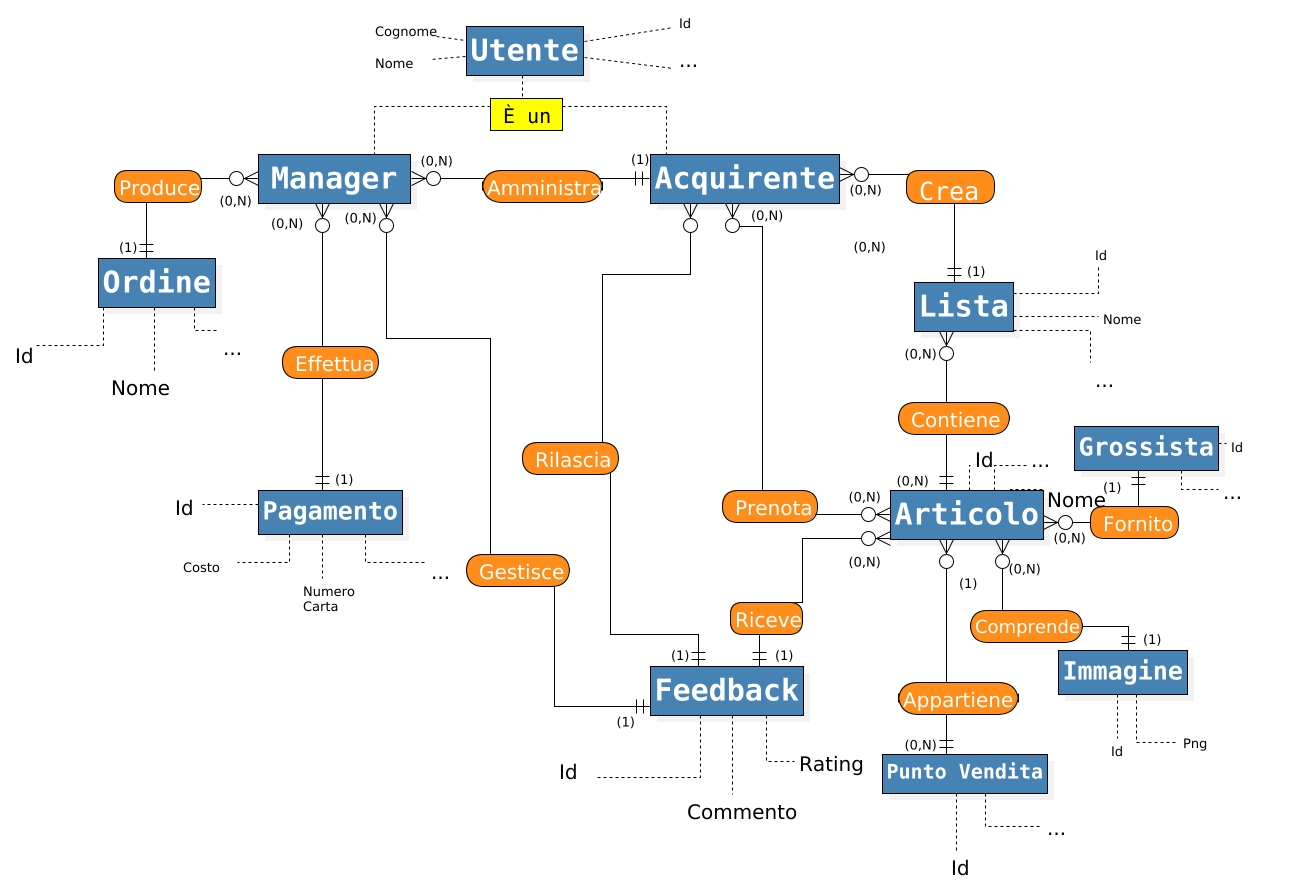
\includegraphics[width=1.3\textwidth]{/Users/matt/Projects/GITHUB/Documentazione/Progettazione concettuale/Progettazione concettuale/progettazione concettuale.jpg}

    \chapter{EER diagram}

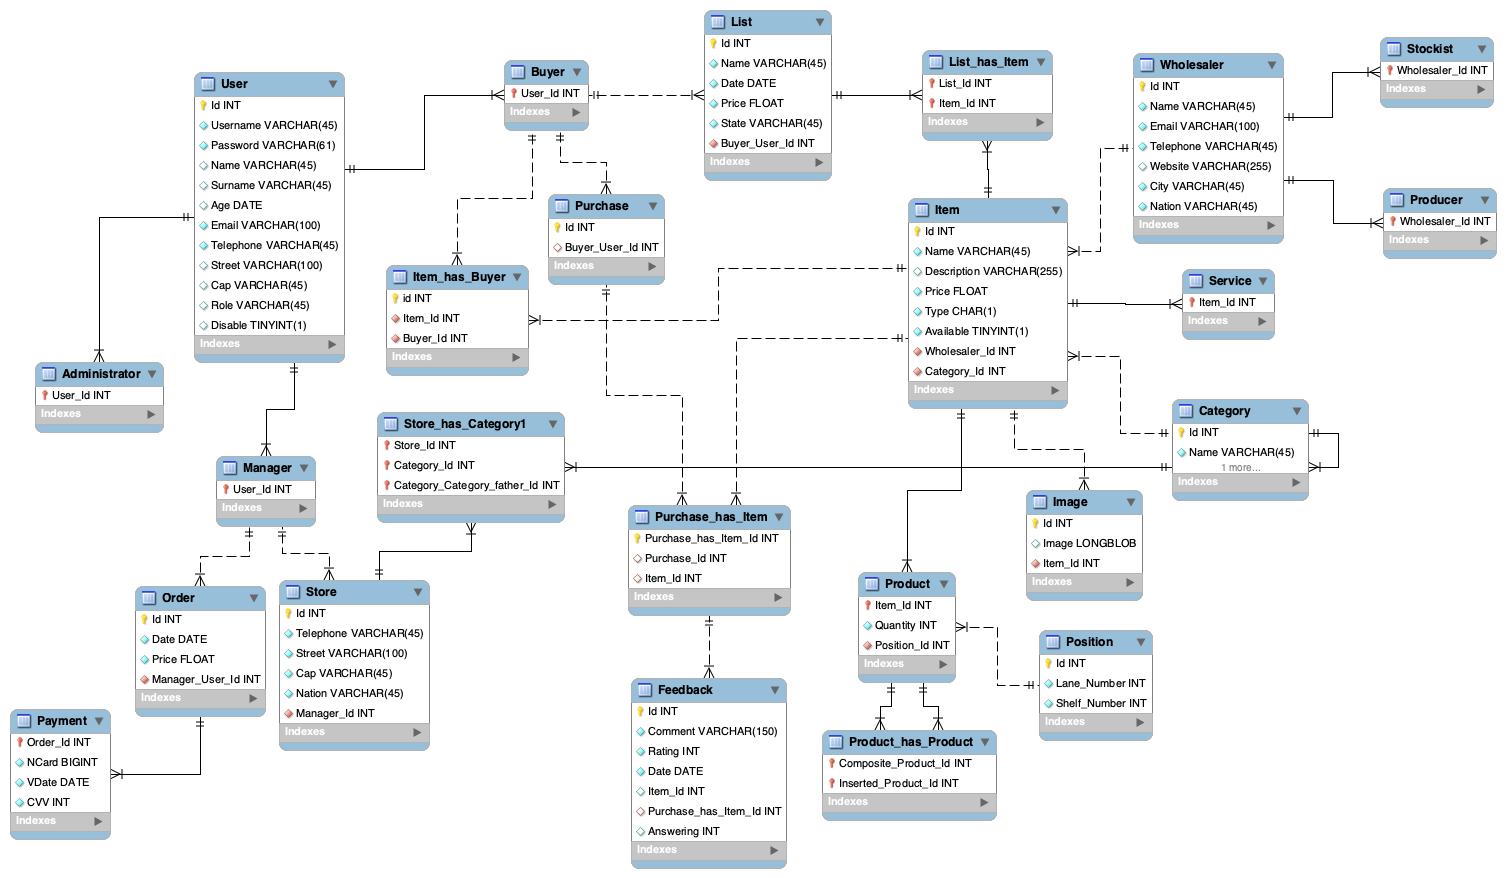
\includegraphics[width=1.3\textwidth]{/Users/matt/Projects/GITHUB/Documentazione/Progettazione concettuale/Progettazione logica/EER diagram.png}

    \chapter{Dizionario dei dati}


\section{Utente}
Descrizione: Entità dell'utente generico
\begin{center}
    \begin{tabular}{||c c c c||}
        \hline
        Attributo & Descrizione & Tipo & (min, max) \\ [0.5ex]
        \hline \hline
        Id &  & int &   \\
        Nome &  & String & (0, 45) \\
        Cognome &  & String & (0, 45) \\
        Età &  & date &  \\
        Email &  & String & (0, 100) \\
        Telefono & & String & (0, 45) \\
        Residenza & Via + numero civico & String & (0, 100) \\
        CAP &  & String & (0, 45) \\
        Professione & Amministratore, Manager, acquirente & char & (1) \\
        \hline
    \end{tabular}
\end{center}


\section{Lista}
Descrizione: Lista d'acquisto del acquirente
\begin{center}
    \begin{tabular}{||c c c c||}
        \hline
        Attributo & Descrizione & Tipo & (min, max) \\ [0.5ex]
        \hline \hline
        Id &  & int &  \\
        Nome &  & String & (0, 45) \\
        Data & Data della creazione & date &  \\
        Costo &  & float &  \\
        \hline
    \end{tabular}
\end{center}

\newpage
\section{Articolo}
Descrizione: Articolo presente nel punto vendita
\begin{center}
    \begin{tabular}{||c c c c||}
        \hline
        Attributo & Descrizione & Tipo & (min, max) \\ [0.5ex]
        \hline \hline
        Id &  & int &  \\
        Nome &  & String & (0, 45) \\
        Descrizione &  & String & (0, 255) \\
        Costo &  & float &  \\
        Categoria &  & String & (0, 45) \\
        Sottocategoria &  & String & (0, 45) \\
        Tipo & Prodotto, composizione, servizio & char &  \\
        \hline
    \end{tabular}
\end{center}


\section{Grossista}
Descrizione: Produttore o fornitore di prodotti o servizi
\begin{center}
    \begin{tabular}{||c c c c||}
        \hline
        Attributo & Descrizione & Tipo & (min, max) \\ [0.5ex]
        \hline \hline
        Id &  & int &  \\
        Nome &  & String & (0, 45) \\
        Email &  & String & (0, 100) \\
        Telefono &  & String & (0, 45) \\
        Sito web &  & String & (0, 255) \\
        Città &  & String & (0, 45) \\
        Nazione &  & String & (0, 45) \\
        \hline
    \end{tabular}
\end{center}


\section{Immagine}
Descrizione: Immagine che permette di vendere l'articolo
\begin{center}
    \begin{tabular}{||c c c c||}
        \hline
        Attributo & Descrizione & Tipo & (min, max) \\ [0.5ex]
        \hline \hline
        Id &  & int &  \\
        Png &  & Image &  \\
        \hline
    \end{tabular}
\end{center}


\section{Punto vendita}
\begin{center}
    \begin{tabular}{||c c c c||}
        \hline
        Attributo & Descrizione & Tipo & (min, max) \\ [0.5ex]
        \hline \hline
        Id &  & int &  \\
        Telefono &  & String & (0, 45) \\
        Residenza & Via + numero civico & String & (0, 100) \\
        CAP &  & String & (0, 45) \\
        Nazione &  & String & (0, 45) \\
        \hline
    \end{tabular}
\end{center}


\section{Feedback}
\begin{center}
    \begin{tabular}{||c c c c||}
        \hline
        Attributo & Descrizione & Tipo & (min, max) \\ [0.5ex]
        \hline \hline
        Id &  & int &  \\
        Commento &  & String & (0, 150) \\
        Rating &  & int & (1, 5) \\
        \hline
    \end{tabular}
\end{center}


\section{Ordine}
Descrizione: Ordine del Manager
\begin{center}
    \begin{tabular}{||c c c c||}
        \hline
        Attributo & Descrizione & Tipo & (min, max) \\ [0.5ex]
        \hline \hline
        Id &  & int &  \\
        Data & Data della creazione & date &  \\
        Costo &  & float &  \\
        \hline
    \end{tabular}
\end{center}


\section{Pagamento}
\begin{center}
    \begin{tabular}{||c c c c||}
        \hline
        Attributo & Descrizione & Tipo & (min, max) \\ [0.5ex]
        \hline \hline
        Id &  & int &  \\
        Data & Data del pagamento & date &  \\
        Costo &  & float &  \\
        NCard & Numero della carta di credito & int & (0, 16) \\
        VData & Data di validità & date &  \\
        CVV & Codice di verifica & inte & (0, 3) \\
        \hline
    \end{tabular}
\end{center}

    \part{Esiti degli unit test}
    \chapter{Unit test}

\section{ListDAOTest}

\includegraphics[width=\textwidth]{/Users/matt/Projects/GITHUB/Documentazione/Unit test/test1.png}

\section{ManagerDAOTest}
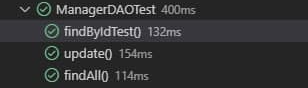
\includegraphics[width=\textwidth]{/Users/matt/Projects/GITHUB/Documentazione/Unit test/test3.png}

\section{OrderDAOTest}

\includegraphics[width=\textwidth]{/Users/matt/Projects/GITHUB/Documentazione/Unit test/test4.png}

\section{CompositeProductDAOTest}

\includegraphics[width=\textwidth]{/Users/matt/Projects/GITHUB/Documentazione/Unit test/test5.png}

\section{PositionDAOTest}

\includegraphics[width=\textwidth]{/Users/matt/Projects/GITHUB/Documentazione/Unit test/test6.png}

\section{ProductDAOTest}
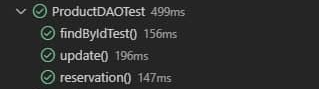
\includegraphics[width=\textwidth]{/Users/matt/Projects/GITHUB/Documentazione/Unit test/test7.png}

\section{PurchaseDAOTest}

\includegraphics[width=\textwidth]{/Users/matt/Projects/GITHUB/Documentazione/Unit test/test8.png}

\section{ServiceDAOTest}

\includegraphics[width=\textwidth]{/Users/matt/Projects/GITHUB/Documentazione/Unit test/test9.png}

\section{StockistDAOTest}

\includegraphics[width=\textwidth]{/Users/matt/Projects/GITHUB/Documentazione/Unit test/test10.png}

\section{StoreDAOTest}
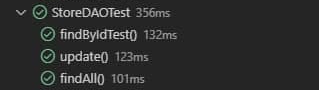
\includegraphics[width=\textwidth]{/Users/matt/Projects/GITHUB/Documentazione/Unit test/test11.png}

\section{WholesalerDAOTest}

\includegraphics[width=\textwidth]{/Users/matt/Projects/GITHUB/Documentazione/Unit test/test12.png}

\section{PaymentDAOTest}

\includegraphics[width=\textwidth]{/Users/matt/Projects/GITHUB/Documentazione/Unit test/test13.png}

\section{ProducerDAOTest}

\includegraphics[width=\textwidth]{/Users/matt/Projects/GITHUB/Documentazione/Unit test/test14.png}

\section{UserDAOTest}

\includegraphics[width=\textwidth]{/Users/matt/Projects/GITHUB/Documentazione/Unit test/test15.png}

\section{BuyerDAOTest}
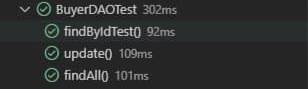
\includegraphics[width=\textwidth]{/Users/matt/Projects/GITHUB/Documentazione/Unit test/test16.jpg}

\section{AdministratorDAOTest}
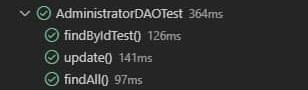
\includegraphics[width=\textwidth]{/Users/matt/Projects/GITHUB/Documentazione/Unit test/test17.jpg}

\section{CategoryDAOTest}

\includegraphics[width=\textwidth]{/Users/matt/Projects/GITHUB/Documentazione/Unit test/test18.jpg}

\section{ItemDAOTest}
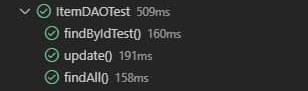
\includegraphics[width=\textwidth]{/Users/matt/Projects/GITHUB/Documentazione/Unit test/test19.jpg}

\section{FeedbackDAOTest}

\includegraphics[width=\textwidth]{/Users/matt/Projects/GITHUB/Documentazione/Unit test/test20.jpg}



    \part{Scrum}
    \chapter{Sprint Backlog}

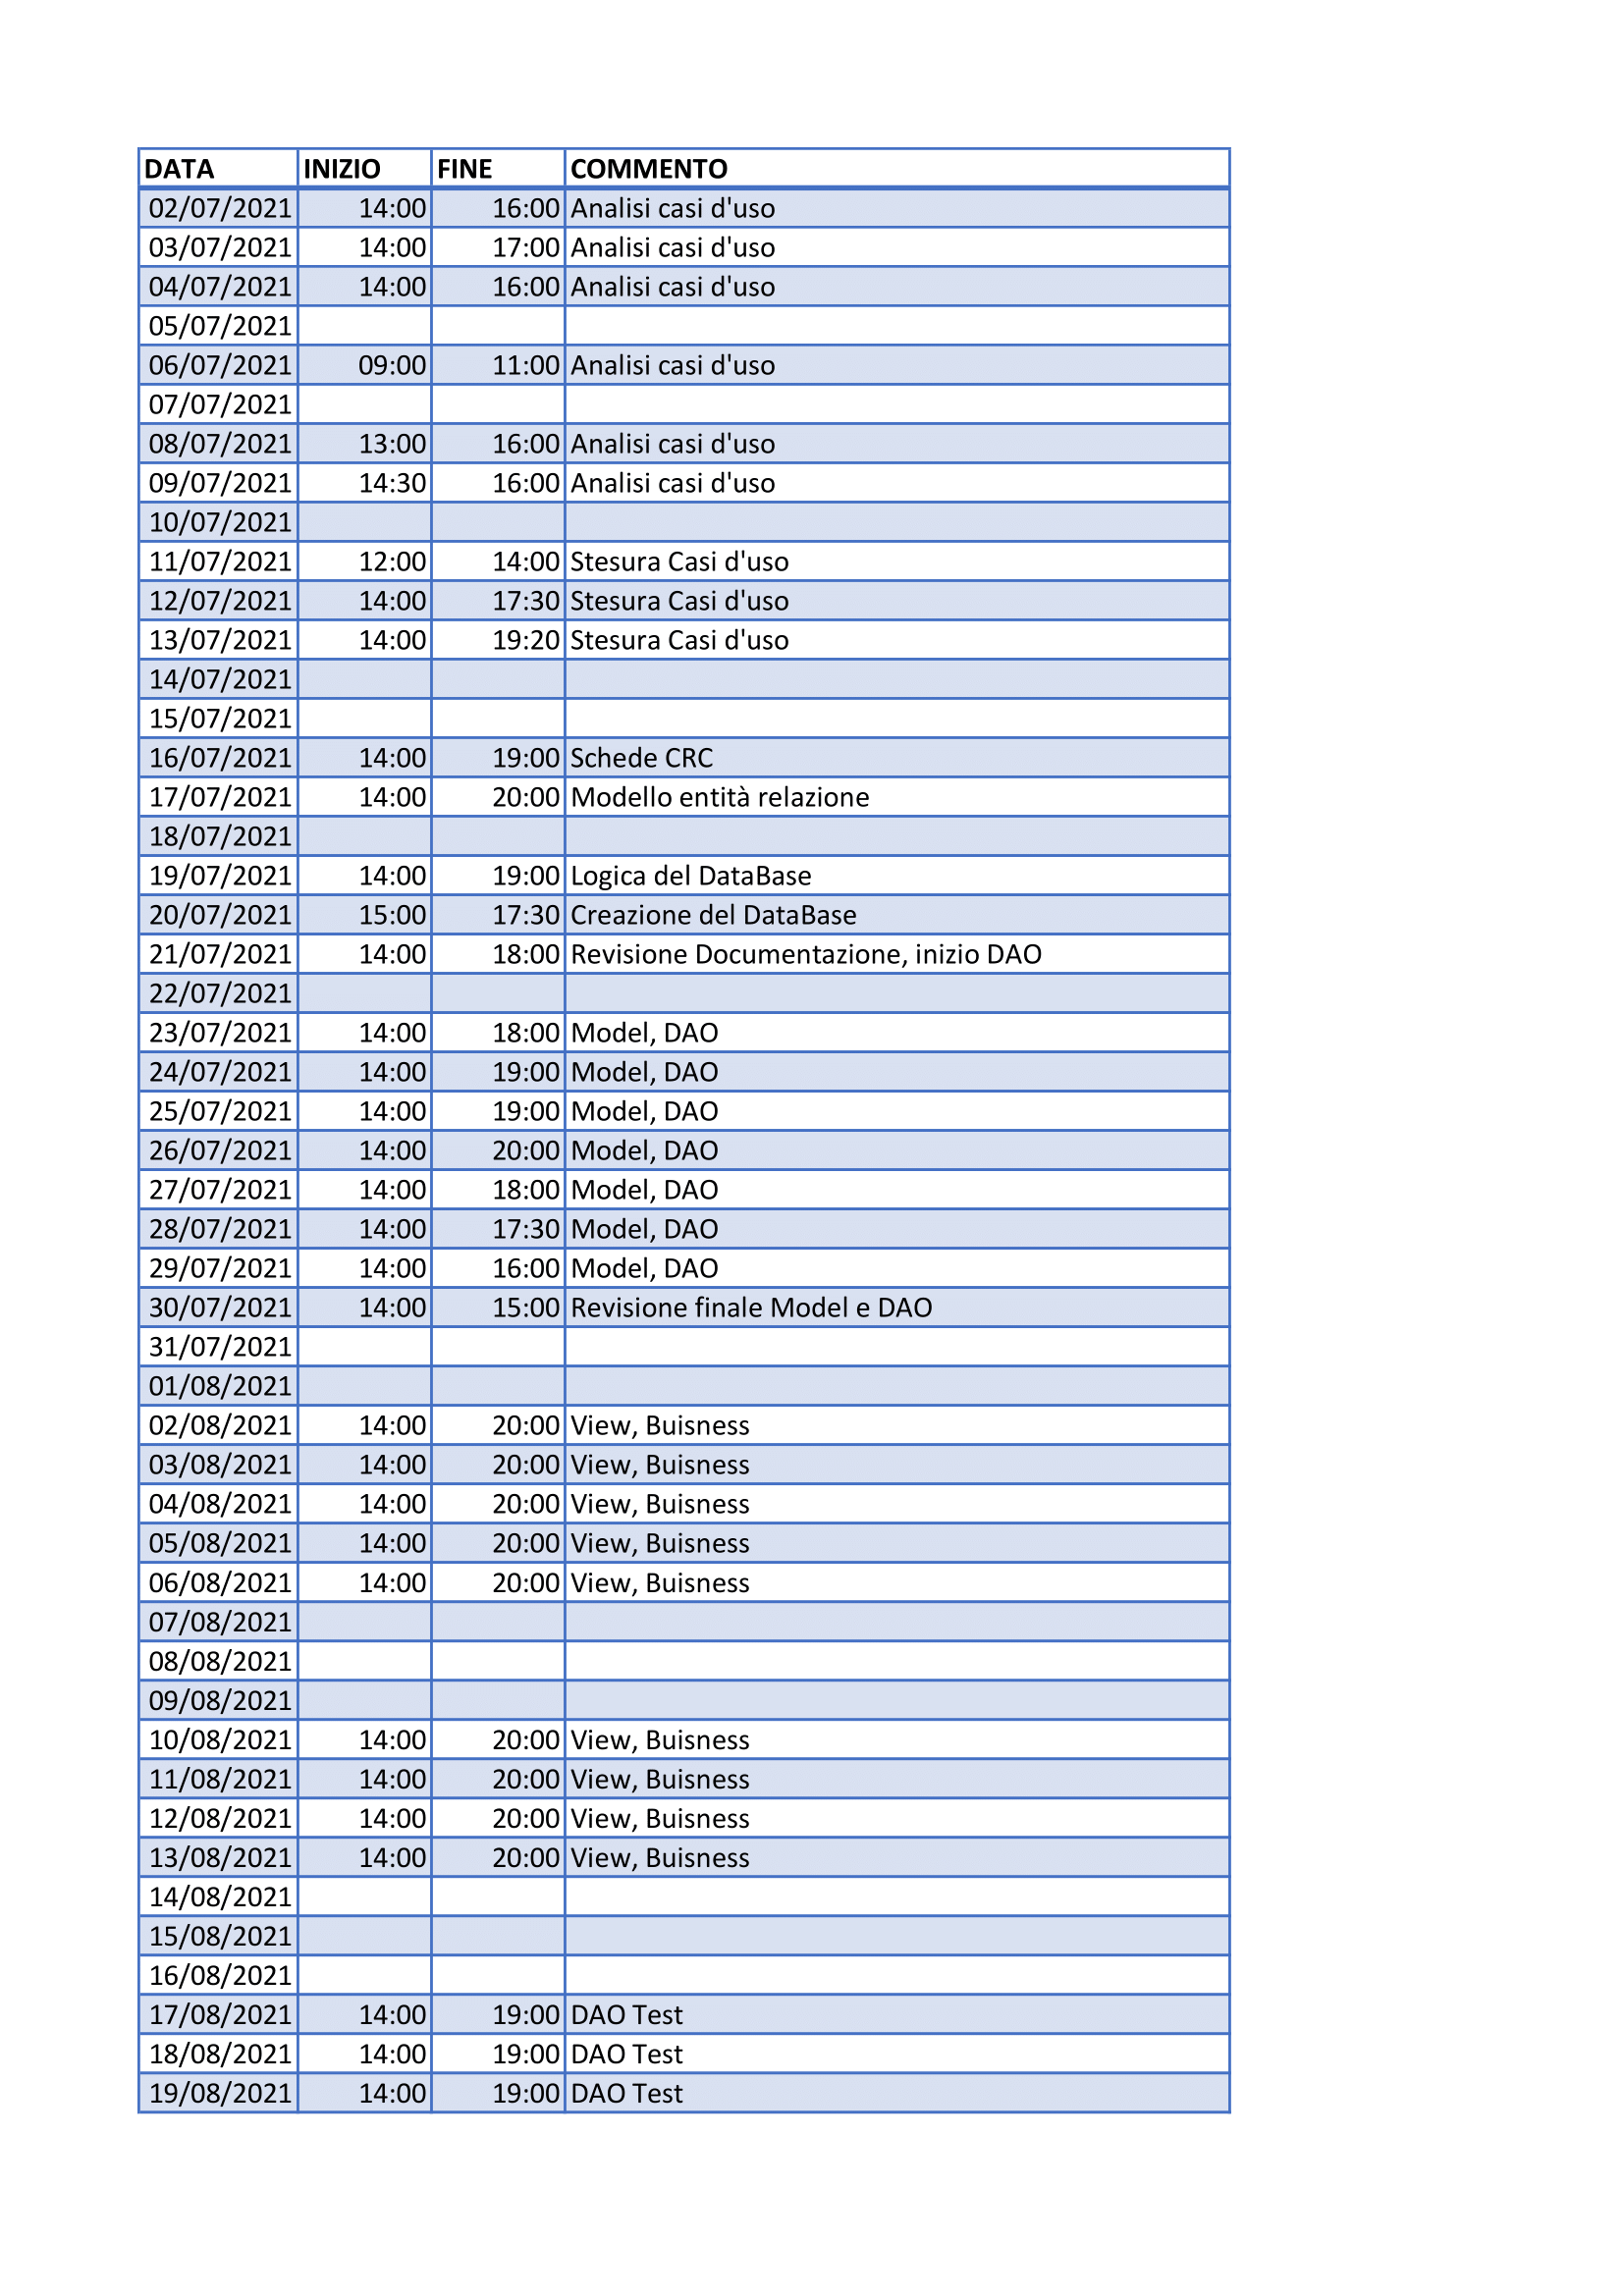
\includegraphics[width=0.75\textwidth]{/Users/matt/Projects/GITHUB/Documentazione/Scrum/Sprint backlog/Sprint BackLog-1.png}

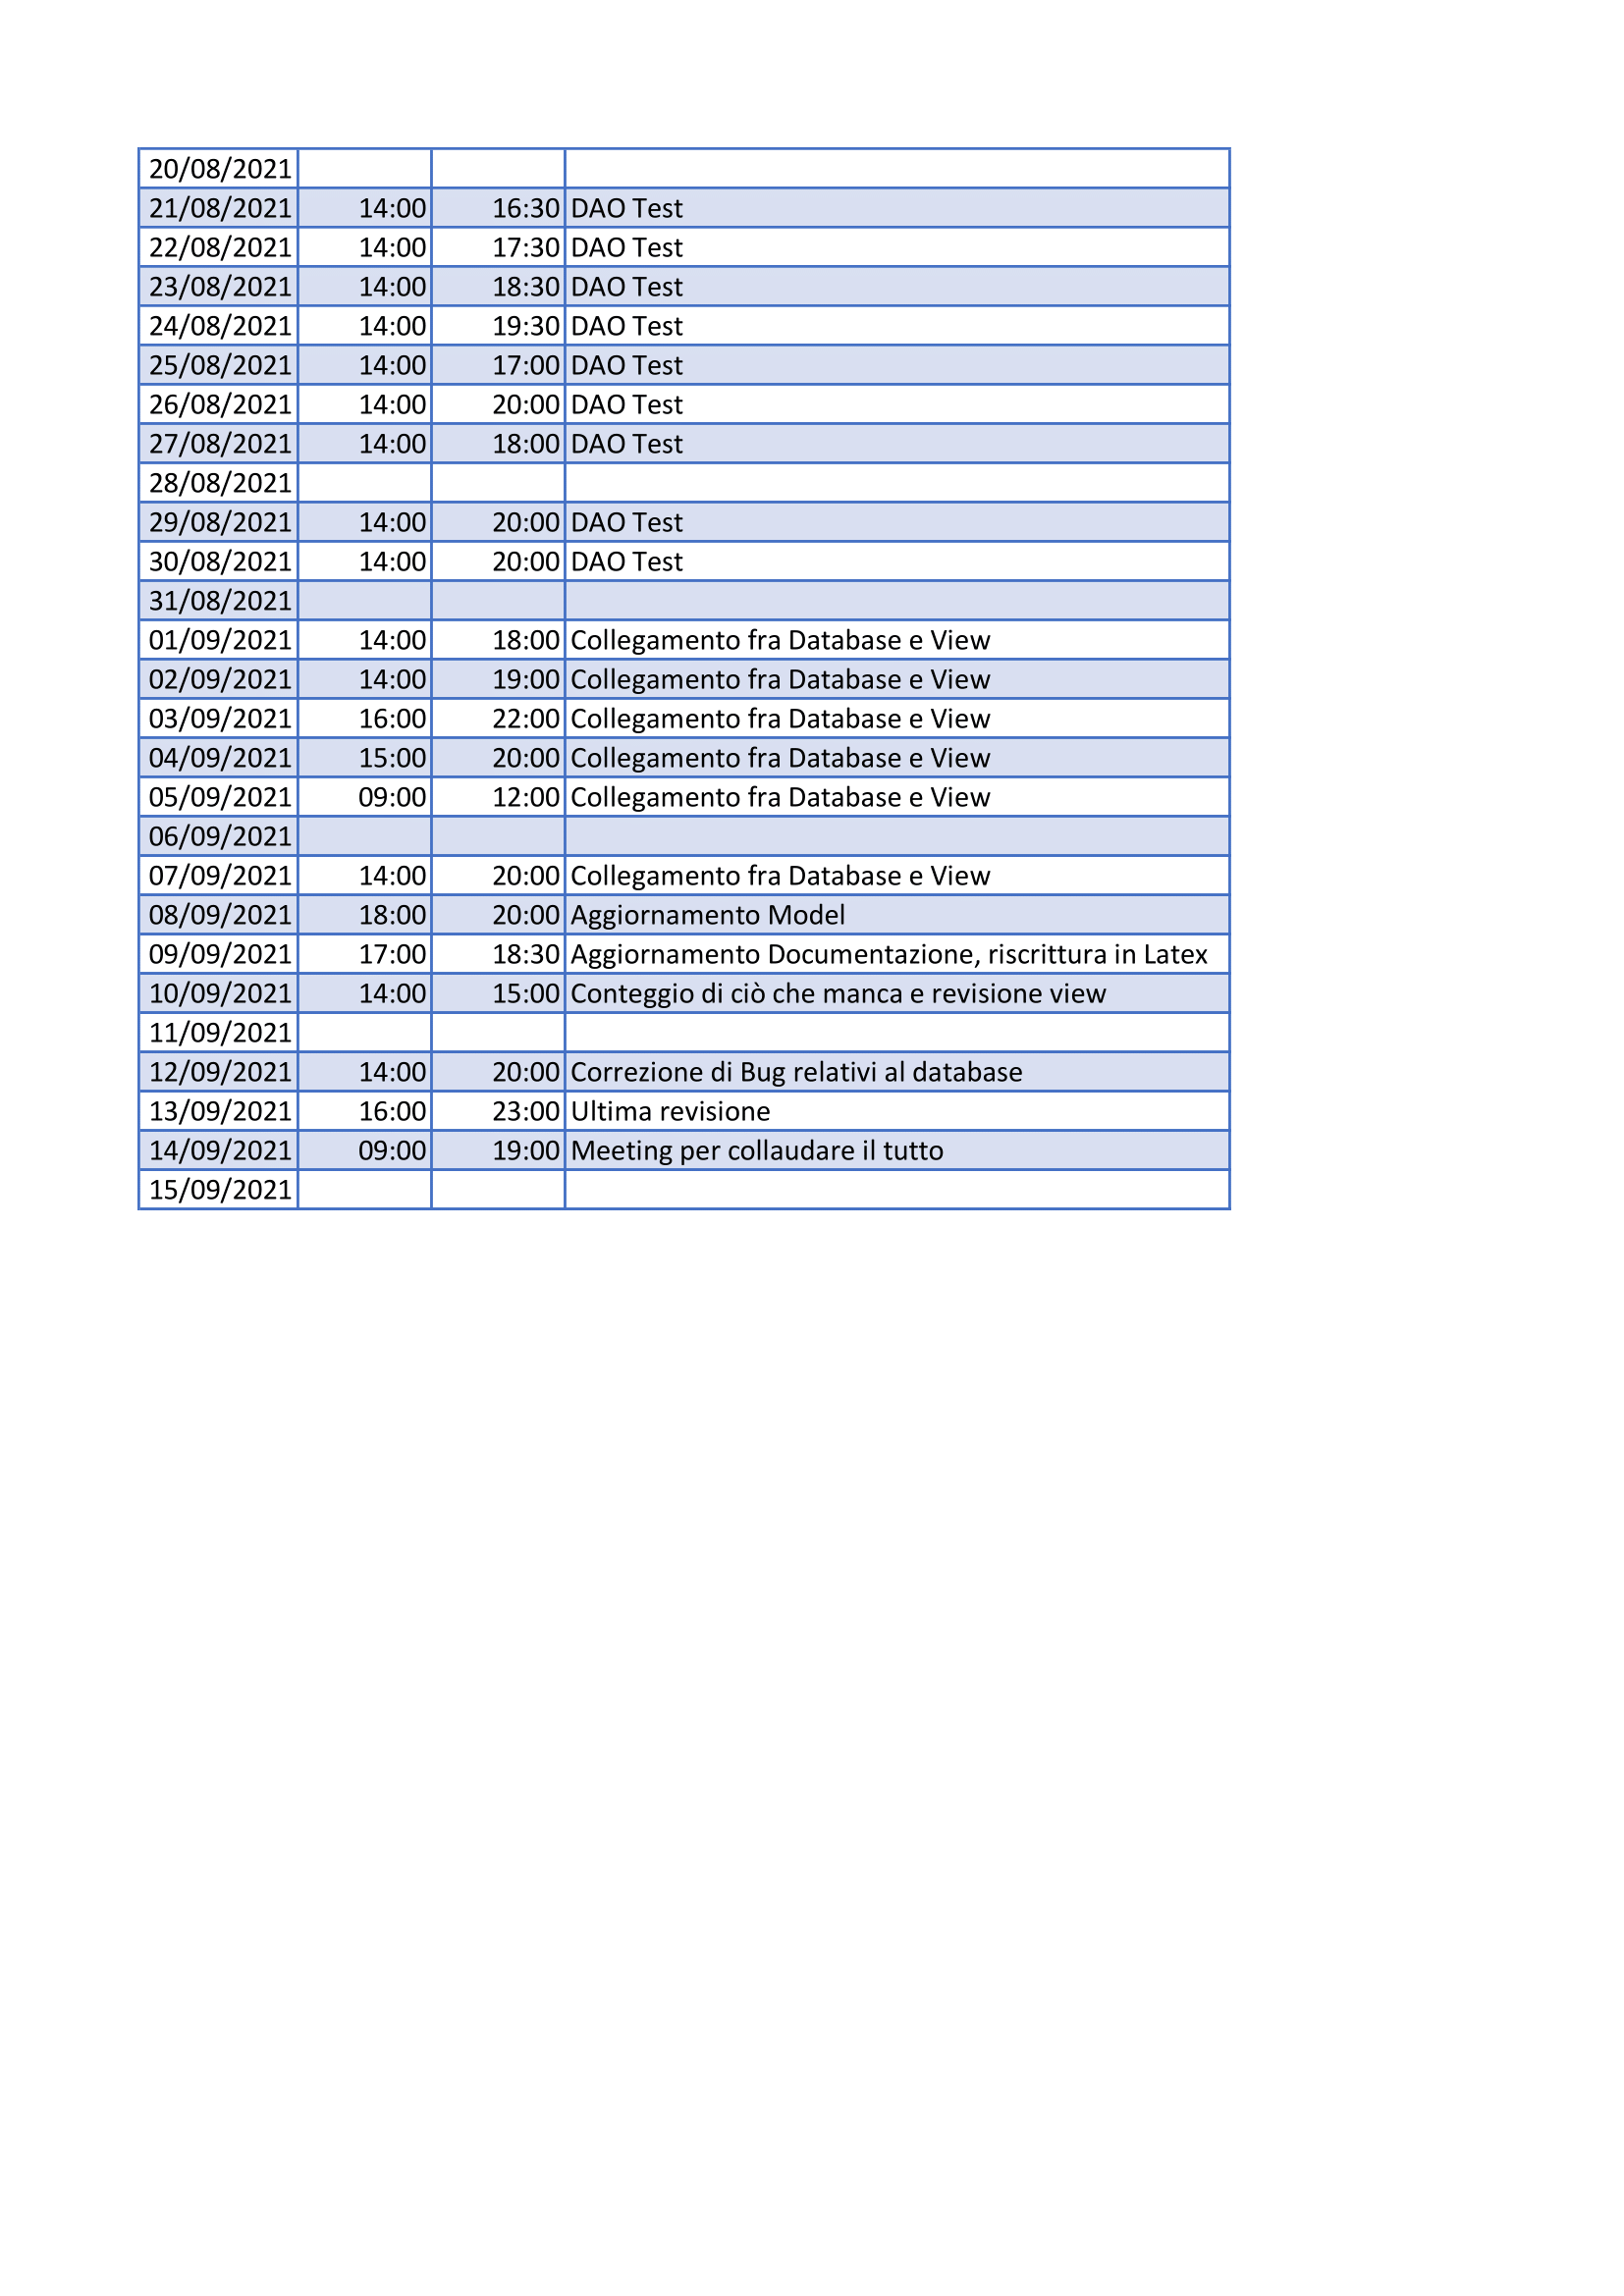
\includegraphics[width=0.75\textwidth]{/Users/matt/Projects/GITHUB/Documentazione/Scrum/Sprint backlog/Sprint BackLog-2.png}


    \chapter{Burndown char}

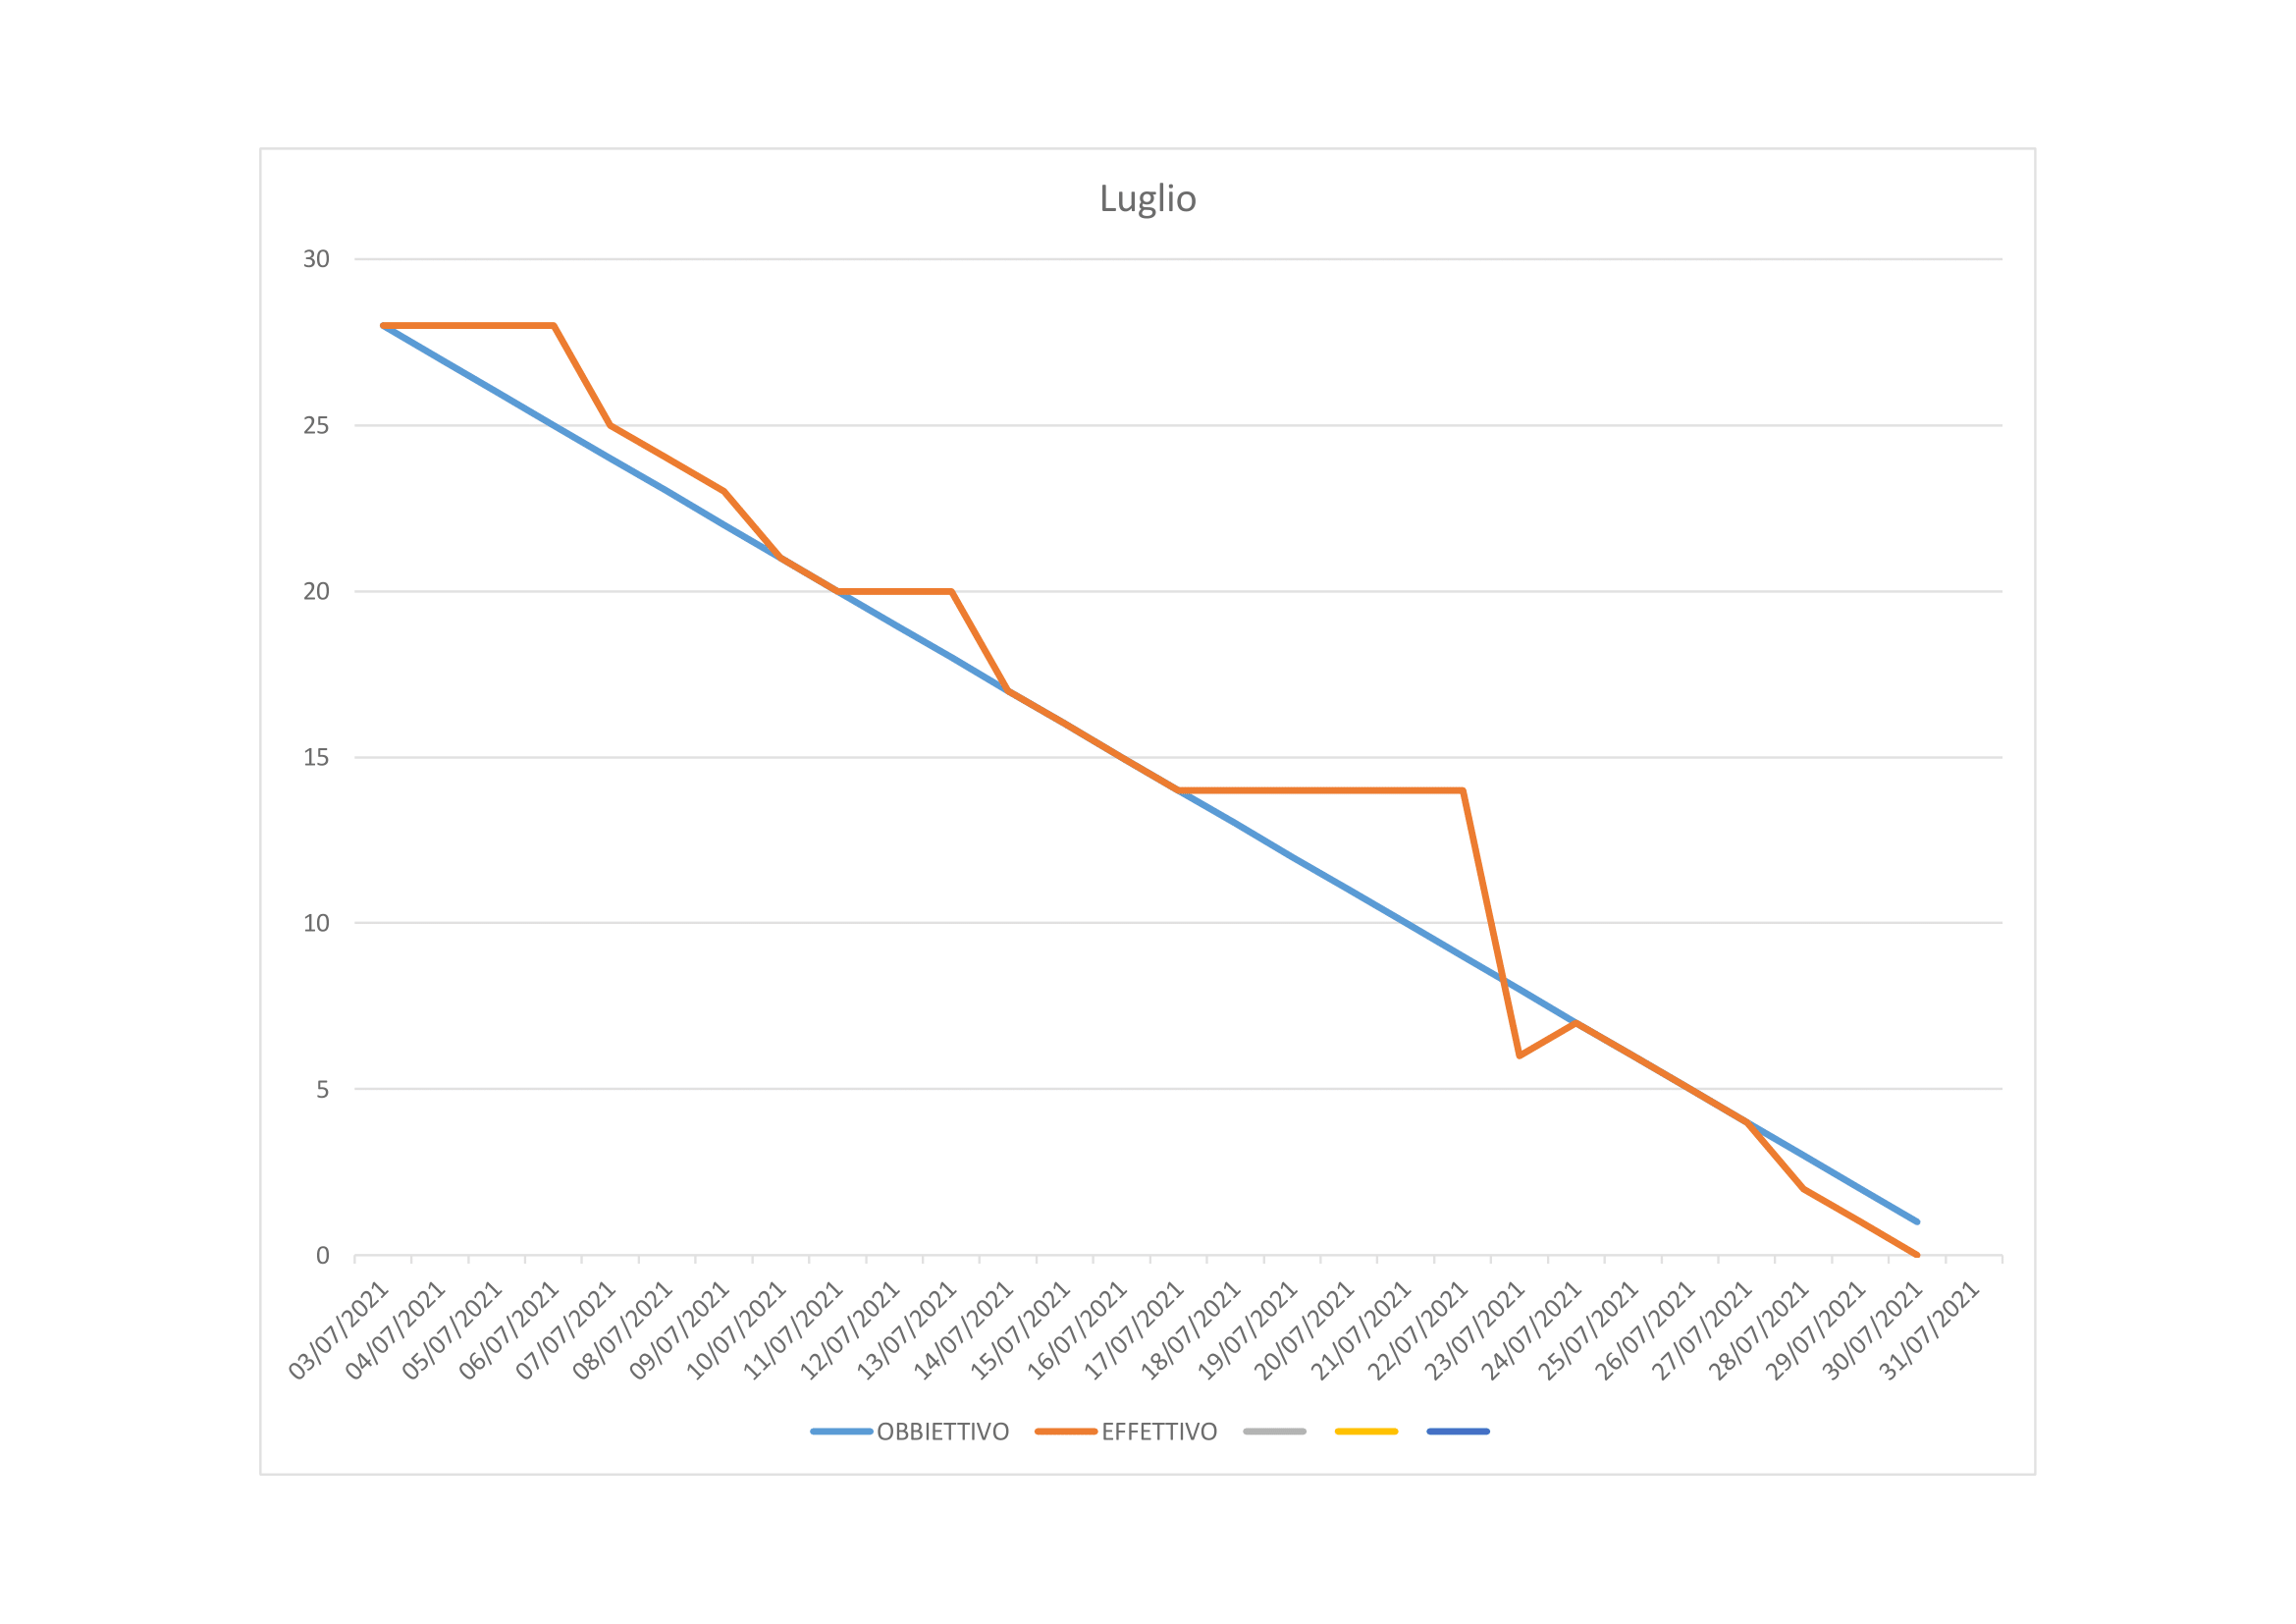
\includegraphics[width=1.3\textwidth]{/Users/matt/Projects/GITHUB/Documentazione/Scrum/Burndown chart/Luglio-1.png}

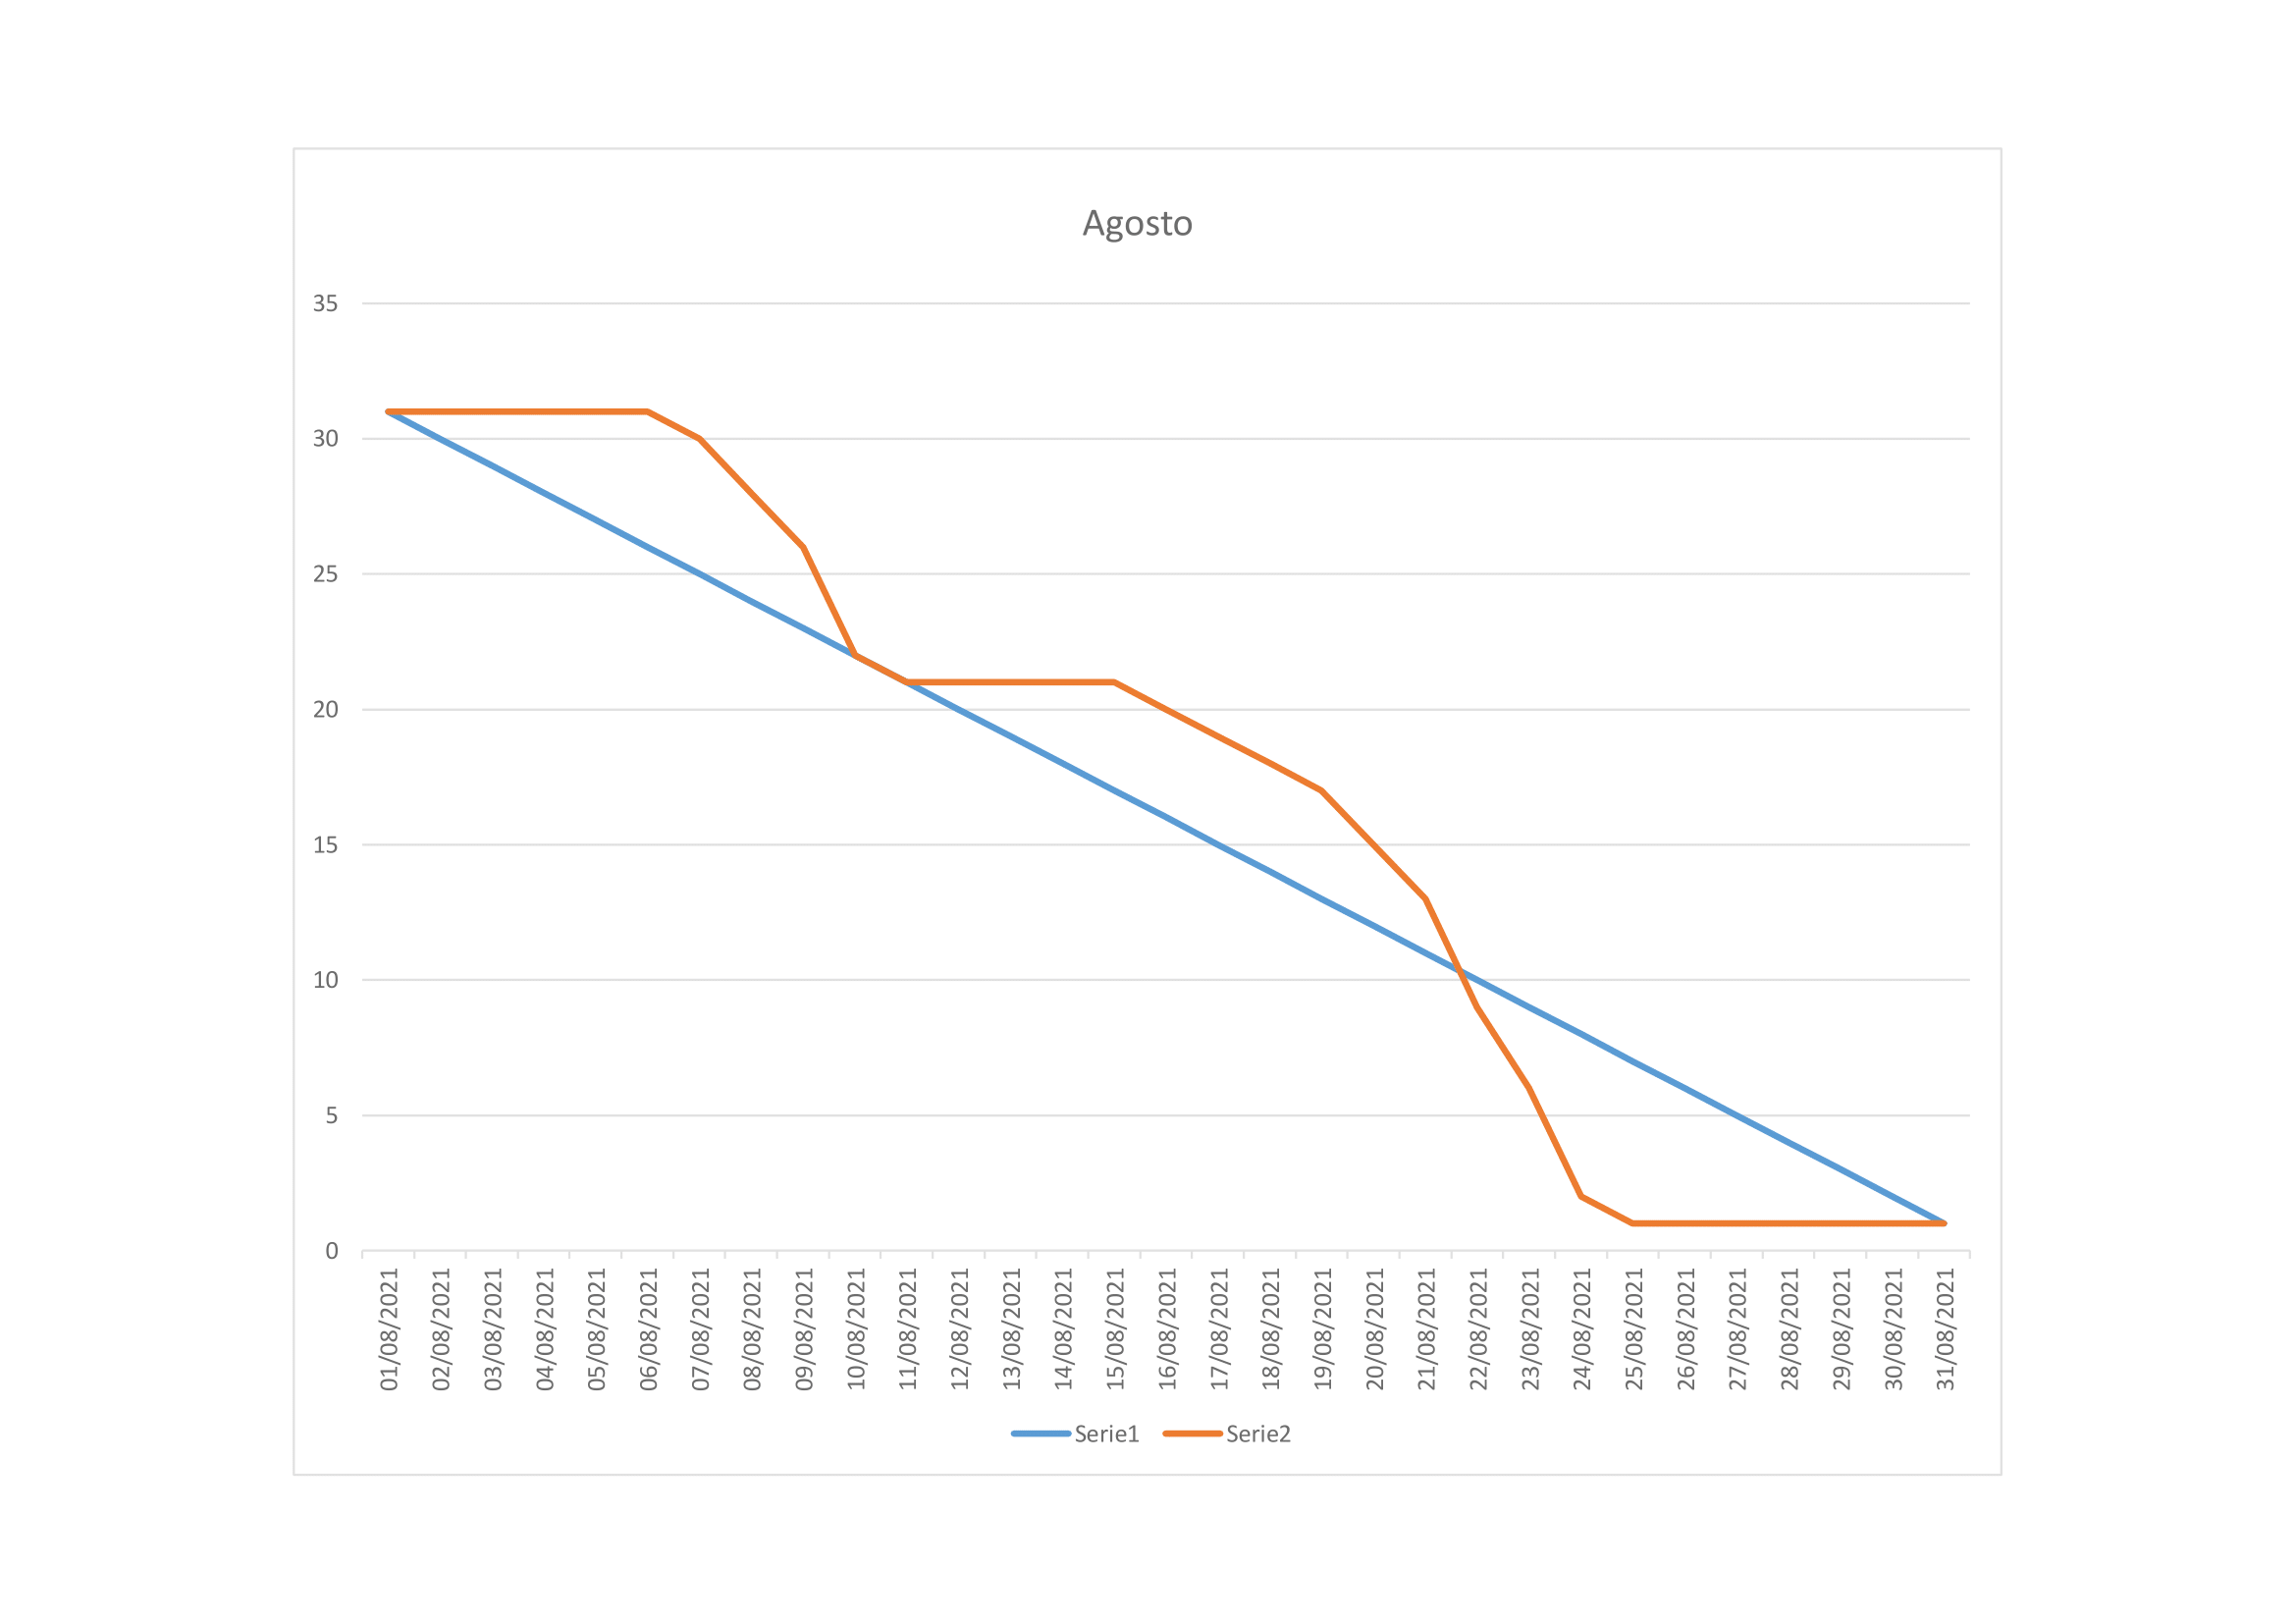
\includegraphics[width=1.35\textwidth]{/Users/matt/Projects/GITHUB/Documentazione/Scrum/Burndown chart/Agosto-1.png}

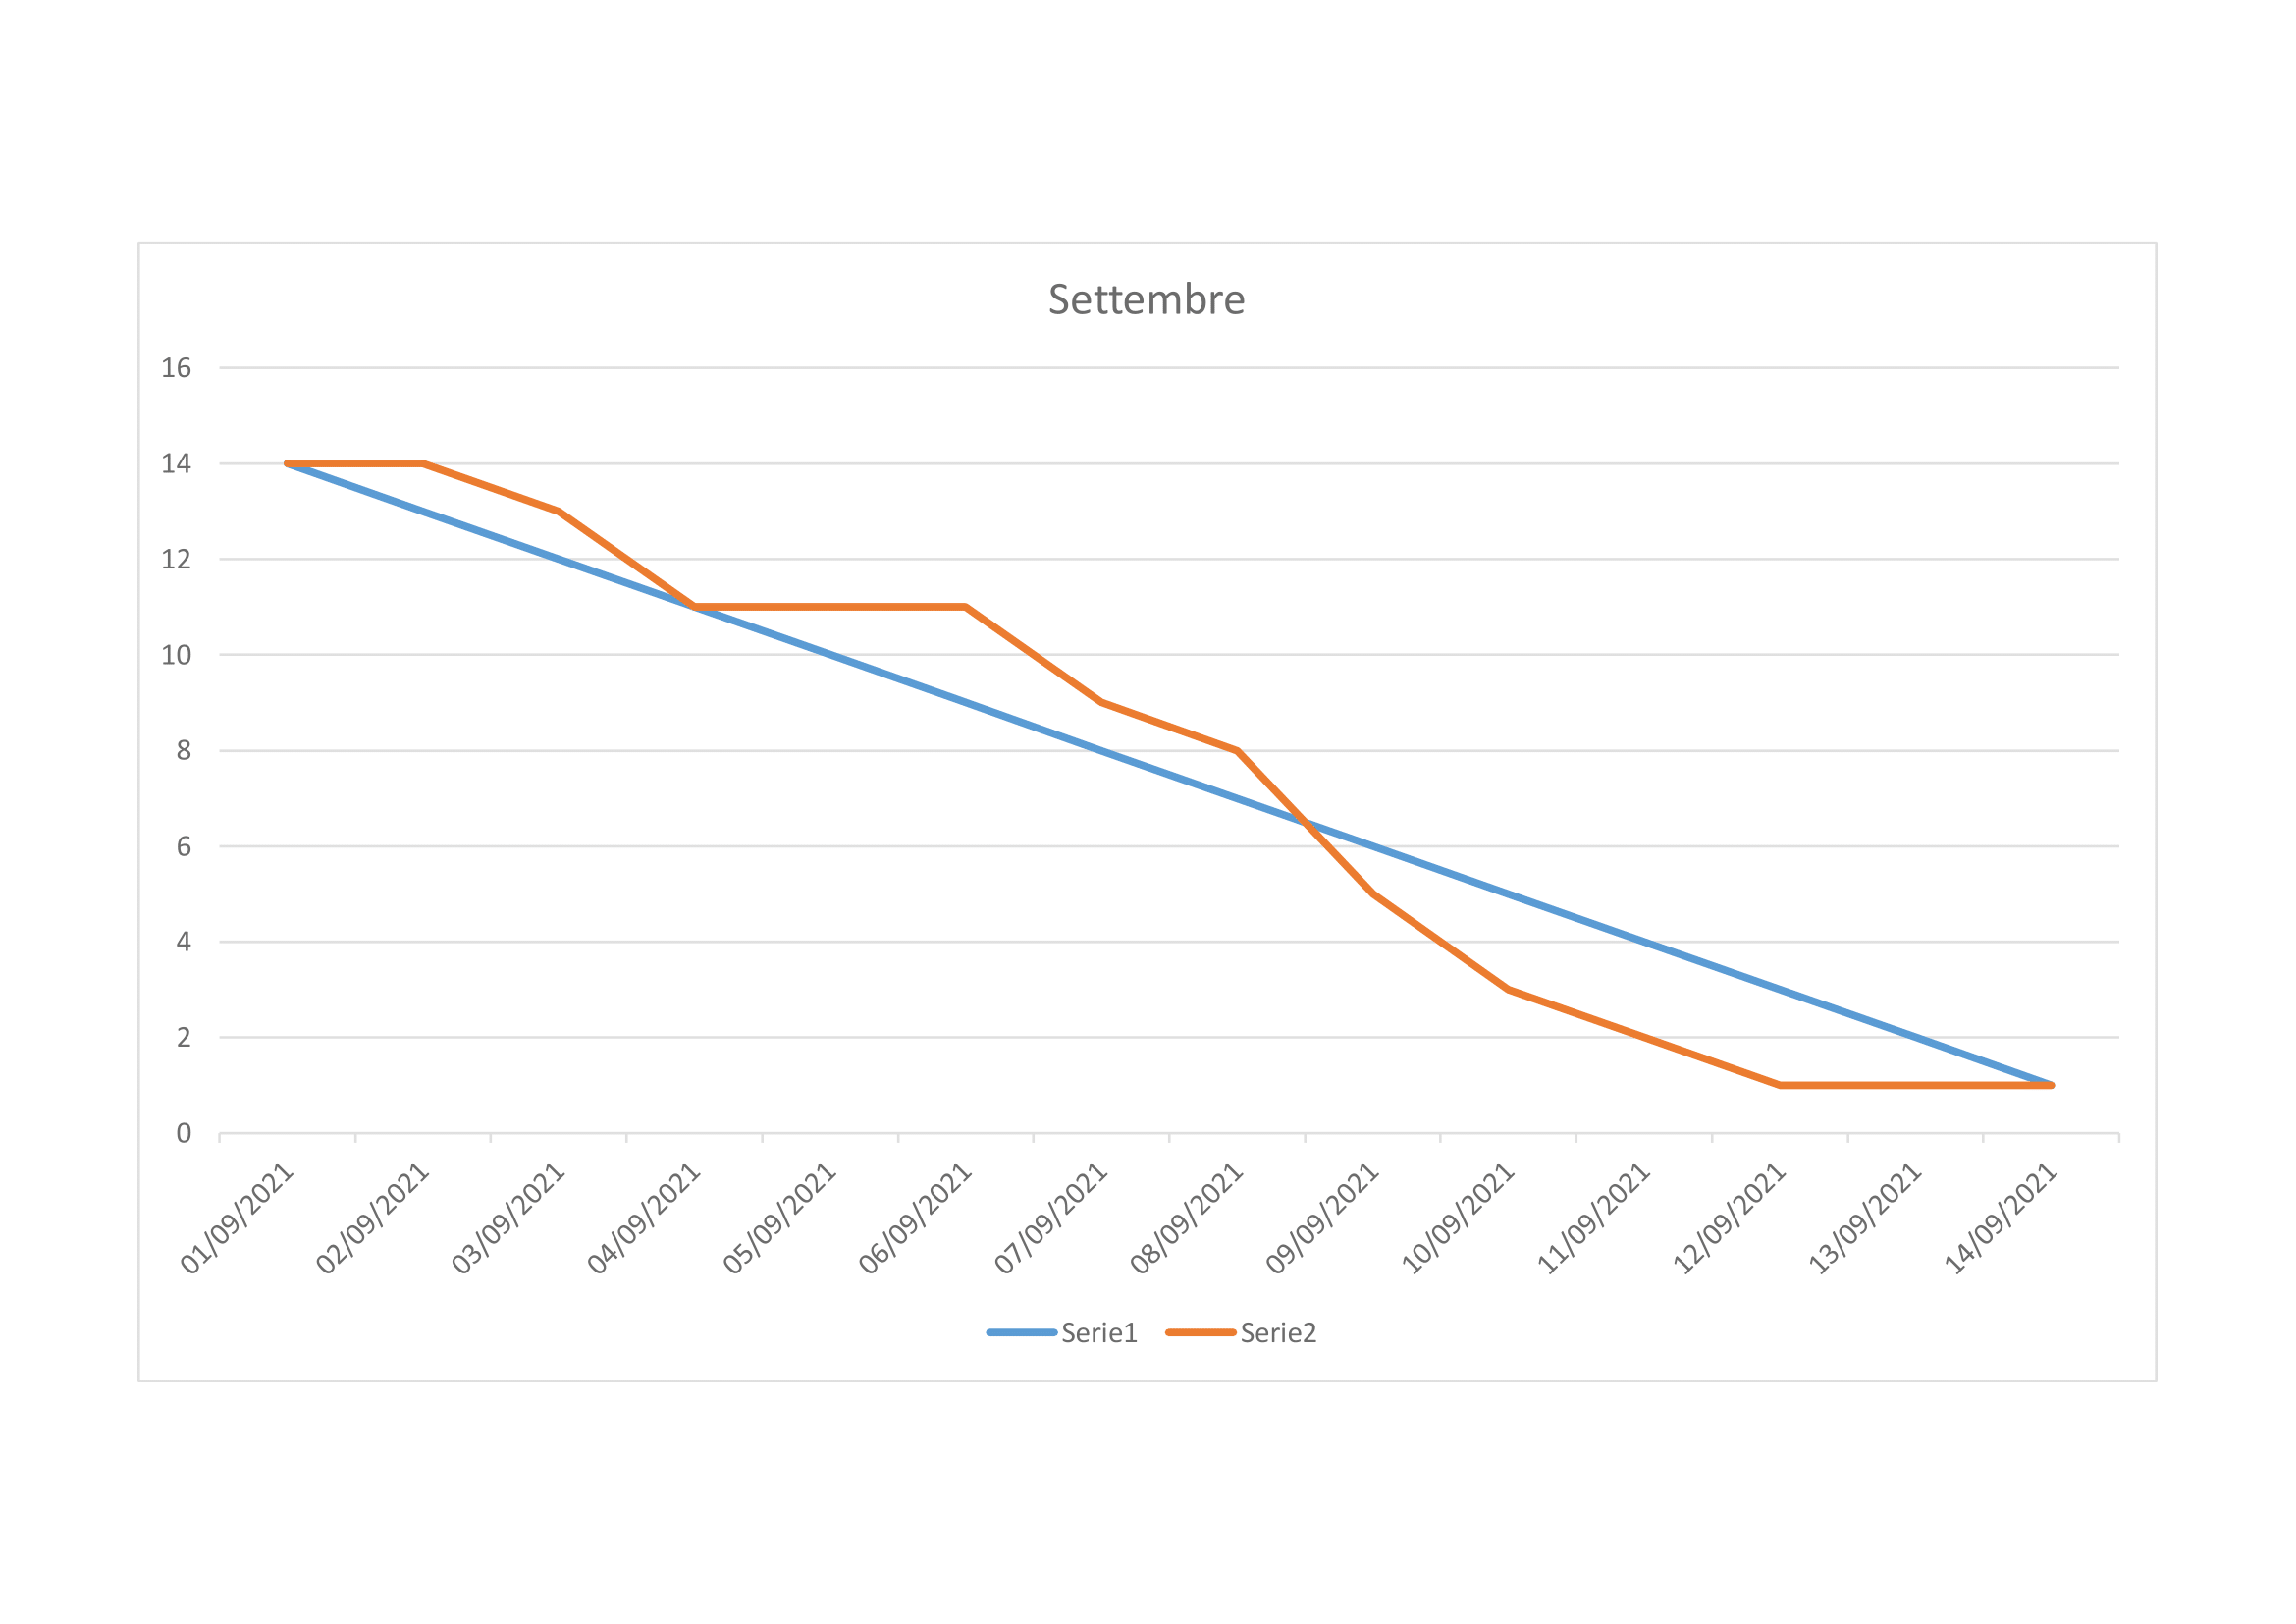
\includegraphics[width=1.3\textwidth]{/Users/matt/Projects/GITHUB/Documentazione/Scrum/Burndown chart/Settembre-1.png}

\end{document}